\documentclass[12pt]{article}
\usepackage{preamble}

\pagestyle{fancy}
\fancyhead[LO,LE]{Физические основы компьютерных \\ и сетевых технологий}
\fancyhead[RO,RE]{Лекции Музыченко Я. Б.}

\fancyfoot[L]{\scriptsize исходники найдутся тут: \\ \url{https://github.com/pelmesh619/itmo_conspects} \Cat}

\renewcommand{\thesection}{}

\begin{document}

    \tableofcontents
    \clearpage

    % begin physics1_2024_09_02.tex

    \section{0. Вводная лекция}

    Задается вопрос: зачем обучающимся программистам нужна физика в учебном плане?

    Приводятся цитаты Л. Богуславского, одного из крупнейших IT инвесторов, и Б. Страуструпа, которые считают,
    что такие фундаментальные дисциплины, как математика, физика, иностранный язык, способствуют развитию
    мышления человека

    Такие компании, как Bell Labs и IBM создали прорывные изобретения в области физики, на основе которых
    построены компьютерные технологии

    В 3-ем семестре курс физики будет состоять из классической механики и основ электричества

    В 4-ом семестре будут темы магнетизма, колебаний, волн и волновых процессов

    В 5-ом семестре будут рассматриваться оптика, основы квантовой физики и квантовые вычисления

    Занятия состоят из лекций, практических и лабораторных занятий.
    Всего в 3-ем семестре будут 5 лабораторных работ


    \section{1. Современная физическая картина мира. Кинематика материальной точки}

        \begin{tcolorbox}[colframe=blue!25, colback=blue!10, title=\textbf{План лекции}]

        \footnotesize
        \begin{itemize}
            \item Историческая справка
            \item Методы и модели в физике
            \item Изучаемые объекты
            \item Физика и другие науки
            \item Фундаментальные взаимодействия
            \item Кинематика материальной точки. Начало
        \end{itemize}
    \end{tcolorbox}



    \textbf{Физика} - раздел естествознания, изучающий свойства и формы движения материи.
    Под материей понимают вещество и поля.

    Научный метод: сначала проводятся наблюдения и эксперименты, из которых выдвигается гипотеза и ищется
    адекватная математическая модель, эта гипотеза проверяется, и если она подтверждается,
    то формируется \textit{теория}

    Пример - открытие Нептуна: в 1781-1845 годах наблюдались аномалии в движении Урана, в 1845 проведение расчетов
    координат новой планеты, а в 1846 обнаружилась новая планета

    Принцип соответствия (Н. Бор, 1923 г.) - каждая новая теория должна включать предыдущую как частный случай

    Изучаемые объекты: вселенная, галактики, звездные системы и планеты, экосистемы, макротела, молекулы, атомы, ядра,
    элементарные частицы

    Всего в физике существуют 4 фундаментальных взаимодействия:

    \begin{tabular}{c|c|c}
        Взаимодействие   & Квант поля & Область взаимодействия                        \\ \hline
        Гравитационное   & гравитон   & масса                                         \\
        Электромагнитное & фотон      & все заряженные частицы, атомы, электротехника \\
        Слабое           & бозон      & радиоактивный распад                          \\
        Сильное          & глюон      & атомные ядра, фундаментальные частицы         \\
    \end{tabular}

    Механика - раздел физики, изучающий механическое движение, то есть движение тел в пространстве и времени.
    Механическое движение тел ОТНОСИТЕЛЬНО.

    \begin{tabular}{c|c|c|}
        & $\ll 3 \cdot 10^8$ м/с & $\approx 3 \cdot 10^8$ м/с \\ \hline
        $\gg 1$ нм & Классическая           & Релятивистская             \\ \hline
        $\ll 1$ нм & Квантовая              & Квантовая теория поля      \\ \hline
    \end{tabular}

    Материальная точка - тело, размерами которого можно пренебречь в условиях данной задачи

    Абсолютно твердое тело (АТТ) - система материальных точек, расстояние между которыми не меняется
    в процессе движения (деформации в процессе движения пренебрежимо малы)

    Тело отсчета - тело, относительно которого определяется положение других тел в пространстве

    Система отсчета - совокупность тела отсчета, связанной с ним системы координат и синхронизированных между собой часов

    % векторный, координатный и естественный способы

    Степени свободы - число независимых скалярных величин, однозначно определяющих положение тела в пространстве

    Материальная точка: $3$ степени свободы

    Система N материальных точек: $3N$ степени свободы

    АТТ: $6$ степеней свободы

    Система единиц (\deutscht{le System International d'unites}), 1960

    $[t] = $ с \quad $[S, l] = $ м

    7 основных единиц:

    $[S] = $ м \quad $[T] = $ К

    $[m] = $ кг \quad $[\nu] = $ моль

    $[t] = $ с \quad $[l] = $ Кд

    $[q] = $ Кл

    Изначально все физические единицы основывались на материальных предметов, из-за которых точности единиц была низкой,
    но недавно все единицы были переопределены на основе физических констант.

    В природе нет абсолютно точных вычислений. Измерение любой физической величины без погрешности не имеет смысла!
% end physics1_2024_09_02.tex

% begin physics1_2024_09_09.tex

    \section{2. Кинематика материальной точки}

    \begin{tcolorbox}[colframe=blue!25, colback=blue!10, title=\textbf{План лекции}]

        \footnotesize
        \begin{itemize}
            \item Основные способы описания движения

            \item Основные понятия кинематики

            \item Кинематика поступательного и вращательного движения

            \item Прямая и обратная задачи кинематики

            \item Численные методы при решении задач
        \end{itemize}
    \end{tcolorbox}

    \Def Кинематика - раздел механики, изучающий движение тел, независимо от причин, вызывающих это движение.

    \Def Траектория - линия, по которой движется материальная точка в пространстве

    \Def Путь - длина траектории

    \Def Перемещение - вектор, проведенный из начальной точки в конечную

    \smallvspace

    \textbf{Способы описания движения}

    \begin{multicols}{3}

        \begin{tcolorbox}
            Векторный способ
        \end{tcolorbox}

        \begin{tcolorbox}
            Координатный способ
        \end{tcolorbox}

        \begin{tcolorbox}
            Естественный (траекторный) способ
        \end{tcolorbox}

    \end{multicols}

    \begin{multicols}{3}

        Положение точки может быть однозначно определено с помощью радиус-вектора

        \smallvspace

        Положение точки может быть однозначно определено с помощью трех скалярных координат

        Положение точки определяется дуговой координатой

        \phantom{.}

    \end{multicols}

    \textbf{Векторный способ}

    $\vec{r_1}, \vec{r_2}$ - радиус-векторы, определяющие положения материальной точки в 1 и 2

    $\Delta \vec{r} = \vec{r_2} - \vec{r_1}$ - перемещение материальной точки

    \Def Скорость - векторная физическая величина, характеризующая быстроту перемещения материальной точки

    Средняя скорость - $\Pair{\vec{v}} = \frac{\Delta \vec{r}}{\Delta t}$

    Мгновенная скорость - $\vec{v} = \lim_{\Delta t \to 0} \frac{\Delta \vec{r}}{\Delta t} = \frac{d \vec{r}}{dt}$

    Средняя путевая скорость - $v_{\text{ср}} = \frac{\Delta S}{\Delta t}$

    \Def Ускорение - векторная физическая величина, характеризующая быстроту изменения скорости материальной точки

    Среднее ускорение - $\Pair{\vec{a}} = \frac{\Delta \vec{v}}{\Delta t}$

    Мгновенное ускорение - $\vec{a} = \lim_{\Delta t \to 0} \frac{\Delta \vec{v}}{\Delta t} = \frac{d \vec{v}}{dt}$

    % годограф скорости

    \textbf{Координатный способ}

    В координатном способе положение точки описано 3 координатами $x, y, z$ (в данном случае в ДПСК)

    $|r| = \sqrt{x^2 + y^2 + z^2}$

    $\vec{r} (t) = r_x (t) \vec{\imath} + r_y (t) \vec{\jmath} + r_z (t) \vec{k} = x(t) \vec{\imath} + y(t) \vec{\jmath} + z(t) \vec{k}$

    $\vec{v} (t) = \frac{d \vec{r}}{dt} = \frac{dx}{dt} \vec{\imath} + \frac{dy}{dt} \vec{\jmath} + \frac{dz}{dt} \vec{k}$

    $\vec{v} (t) = v_x(t)\vec{\imath} + v_y(t) \vec{\jmath} + v_z(t) \vec{k}$

    $|\vec{v}| = \sqrt{v_x^2 + v_y^2 + v_z^2}$


    % ускорение

    Прямая задача:

    $\vec{r}(t), x(t), y(t), z(t) \longrightarrow \vec{v}(t), \vec{a}(t), v_x, v_y, v_z, a_x, a_y, a_z$

    Решением является дифференцирование

    Обратная задача:

    $\vec{a}(t), a_x, a_y, a_z \longrightarrow \vec{v}(t), \vec{r}(t), x(t), y(t), z(t)$

    Для обратной задачи решением является интегрирование

    $\vec{v} = \frac{d\vec{r}}{dt} \quad d\vec{r} = \vec{v}dt \quad \Delta\vec{r} = \int_{t_1}^{t_2} \vec{v}dt$

    \begin{tcolorbox}
        $\vec{r} = \vec{r_0} + \Delta \vec{r} = \vec{r_0} + \int_{t_1}^{t_2} \vec{v}dt$
    \end{tcolorbox}

    Аналогично для ускорения

    Численное решение ОДУ (обыкновенного дифференциального уравнения) $\frac{dy}{dx} = f(x, y)$ на отрезке $[x_0, x_n]$ при условии $y(x_0) = y_0$

    Разбиваем отрезок $[x_0, x_n]$ на конечное число частей введением узловых точек

    Шаг разбиения: $h = \frac{x_N - x_0}{N}$

    По определению производной $\frac{dy}{dx} = \frac{y_{i + 1} - y_i}{h}$, из этого:

    \begin{tcolorbox}
        Формула Эйлера: $y_{i + 1} = y_i + hf(x_i, y_i)$
    \end{tcolorbox}

    $dy = f(x, y) dx$

    $\Delta y = y_{i + 1} - y_i = \int_{x_i}^{x_{i + 1}} f(x, y) dx$

    \textbf{Естественный (траекторный) способ}

    Если траектория точки заранее известна, то положение точки задается дуговой координатой $l(t)$

    $\vec{v} = v_\tau \vec{\tau} \quad v_\tau \frac{dl}{dt} |\vec{\tau}| = 1$

    $\vec{a} = \frac{d\vec{v}}{dt} = \frac{dv_\tau}{dt} \vec{\tau} + \frac{d\vec{\tau}}{dt} v_\tau \quad\quad\quad \frac{d\tau}{dt} = \frac{d\tau}{dl} \cdot \frac{dl}{dt} = \frac{d\tau}{dl} v_\tau$

    $\vec{a} = \frac{d\vec{v}}{dt} = \frac{dv_\tau}{dt} \vec{\tau} + \frac{d\vec{\tau}}{dt} v_\tau^2 $

    $d\tau = \tau d\alpha$

    $dl = R d\alpha \quad\quad\quad d\vec{\tau} \uparrow\uparrow \vec{n}$

    $R$ - радиус кривизны траектории

    $\vec{\alpha} = \frac{dv_\tau}{dt} \vec{\tau} + \frac{1}{R} v_\tau^2 \vec{n} \quad\quad\quad \vec{a} = \vec{a_\tau} + \vec{a_n}$

    Тангенциальное ускорение отвечает за изменение модуля скорости, направлено по касательной к траектории движения

    Нормальное ускорение отвечает за изменение направления вектора скорости, направлено к центру кривизны траектории
% end physics1_2024_09_09.tex

% begin physics1_2024_09_16.tex

    \section{3.
    Кинематика вращательного движения.
    Динамика материальной точки}

    \begin{tcolorbox}[colframe=blue!25, colback=blue!10, title=\textbf{План лекции}]

        \footnotesize
        \begin{itemize}
            \item Угловые величины: угол поворота, угловая скорость

            \item Взаимосвязь между линейными и угловыми величинами

            \item Плоское движение

            \item Динамика материальной точки

            \item Законы Ньютона. Силы в механике

            \item Принципы работы акселерометра
        \end{itemize}
    \end{tcolorbox}

    \subsection{Движение по окружности}

    Возьмем точку $A$, положение которое определим через $\vec{r}$. Точка $A$ движется по окружности вокруг неподвижной оси $OO^\prime$

    Тогда $d\vec{r}$ - перемещение, $d\vec{\varphi}$ - элементарный угол поворота (вектор определяет в какую сторону, по часовой или против,
    обращается по окружности тело; вектор направлен перпендикулярно окружности)

    $|d\vec{r}| = Rd\varphi = r \cdot \sin \alpha d \varphi$

    $R = r \cdot \sin \alpha$

    $d\vec{r} = [d \vec{\varphi} \vec{r}]$ \hfill {\scriptsize здесь и далее $[\vec{x}\vec{y}]$ - векторное произведение}

    Угловая скорость - векторная величина, показывающая как меняется угол поворота тела со временем: $\Pair{\omega} = \frac{\Delta \varphi}{\Delta t} \quad\quad\quad \vec{\omega} = \frac{d\vec{\varphi}}{dt}$

    Направление совпадает с направлением угла поворота $d\vec{\varphi}$: $\vec{\omega} \uparrow\uparrow d\vec{\varphi}$

    Угловое ускорение - векторная величина, показывающая как меняется угловая скорость тела со временем

    $\Pair{\beta} = \frac{\Delta \omega}{\Delta t} \quad\quad \vec{\beta} = \frac{d\vec{\omega}}{dt} = \frac{d^2 \vec{\varphi}}{dt^2}$

    Направление совпадает с направлением вектора изменения скорости $\Delta \vec{\omega}$: $\vec{\beta} \uparrow\uparrow d\vec{\omega}$

    $d\vec{r} = [d\vec{\varphi} \vec{r}]$

    $dr = d\varphi \cdot r \cdot \sin \alpha = d\varphi \cdot R$

    Выразим скорость $\vec{v} = \frac{d\vec{r}}{dt} = [\frac{d\vec{\varphi}}{dt}\vec{r}] = [\vec{\omega} \vec{r}]$

    $v = \omega \cdot r \cdot \sin \alpha = \omega \cdot R$

    Выразим ускорение: $\vec{a} = \frac{d\vec{v}}{dt} = [\frac{d\vec{\omega}}{dt} \vec{r}] + [\vec{\omega} \frac{d\vec{r}}{dt}] = [\vec{\beta}\vec{r}] + [\vec{\omega}\vec{v}] = \vec{a}_\tau + \vec{a}_n$

    $\vec{a}_\tau$ называют тангенциальным ускорением (напраленным по касательной), $\vec{a}_n$ - нормальным (направленным к центру)

    $a_\tau = \beta \cdot r \cdot \sin\alpha = \beta \cdot R$

    Перемещение, путь, скорость:

    \begin{multicols}{2}

        $d\vec{r} = [d\vec{\varphi} \vec{\rho}] (\vec{\rho}\text{ - вектор радиуса окружности})$

        $dr = d\varphi \cdot R$

        $S = \varphi \cdot R$

        $\vec{v} = [\vec{\omega} \vec{\rho}]$

        $v = \omega \cdot R$

    \end{multicols}

    Ускорение: $\vec{a} = [\vec{\beta}\vec{r}] + [\vec{\omega}\vec{v}]$

    \begin{multicols}{3}

        $\vec{a}_\tau = [\vec{\beta}\vec{r}]$

        $a_\tau = \beta \cdot R$

        $\vec{a}_n = [\vec{\omega}\vec{v}] = [\vec{\omega}[\vec{\omega}\vec{\rho}]]$

        $a_n = \omega^2 R = \frac{1}{R} v^2$

        $T = \frac{2\pi}{\omega} = \frac{1}{\nu}$ - период

        $\nu = \frac{\omega}{2\pi} = \frac{1}{T}$ - частота

    \end{multicols}

    Плоское движение - движение твердого тела, при котором каждая его точка движется в плоскости,
    параллельной некоторой неподвижной в данной системе отсчета плоскости

    $\vec{r} = \vec{r}_0 + \vec{r}^\prime$

    $d\vec{r} = d\vec{r}_0 + d\vec{r}^\prime = d\vec{r}_0 + [d\vec{\varphi}\vec{r}]$

    $\vec{v} = \vec{v}_0 + [\vec{\omega}\vec{r}]$

    $\vec{v}_C$ - скорость центра колеса относительно точки отсчета

    $\vec{v}_{\text{вр}}$ - скорость точек колеса относительное его центра

    \Def Динамика - раздел механики, изучающий причины, вызывающие движение тел

    1687 г. - законы Ньютона, основа классической механики (механики Ньютона), обобщение большего количества опытов (Г. Галилей)

    Классическая механика - частный случай  1) СТО при скоростях много меньших скорости света $v \ll c$;
    2) квантовой механики при массах, много больших массы атома

    В динамике существуют различия между системами отсчета и преимущества одних СО над другими.

    Существуют такие системы отсчета, относительно которых свободное тело (тело, на которое не действуют другие тела) движется равномерно
    и прямолинейно или находится в состоянии покоя. Таким системы называются инерциальными (ИСО)

%    Земля $a_n = 3.4 \frac{\text{см}}{\text{с}^2}$
%
%    Центр Земли $a_n = 0.6 \frac{\text{см}}{\text{с}^2}$
%
%    Земля $a_n = 3 \cdot 10^{-8} \frac{\text{см}}{\text{с}^2}$
    % for later use i think

    \mediumvspace

    \textbf{Принцип относительности Галилея:}

    Любая СО, движущаяся с постоянной скоростью относительно ИСО, также является ИСО. Тогда справедливо любое из этих утверждений:

    \begin{enumerate}
        \item все ИСО эквивалентны друг другу по своим механическим свойствам
        \item во всех ИСО свойства пространства и времени одинаковы
        \item законы механики одинаковы во всех ИСО
    \end{enumerate}

    % сложное движение земли
    % перечитываю это и не понимаю, че было

    Преобразования Галилея - преобразования координат при переходе от одной ИСО к другой

    $K, K^\prime$ - ИСО

    $\vec{V}$ - скорость, с которой движется СО $K^\prime$ относительно $K$
    $t = t^\prime$

    $\vec{r} = \vec{r}^\prime + \vec{V}t$

    $\vec{c} = \vec{v}^\prime + \vec{V}$

    $\vec{a} = \vec{a}^\prime$

    \Def Сила - физическая величина, определяющая количественную характеристику и напраление воздействия, оказываемого на данное тело
    со стороны других тел.

    Силы условно можно разделить на силы, возникающие при непосредственном контакте (силы трения, давления) и на силы,
    возникающие через поля (электрические, гравитационные).

    \Def Инертная масса - мера инертности тела, то есть способности тела сохранять свою скорость при движении

    \Def Гравитационная масса - мера гравитацонного взаимодействия, величина, определяющая вес тел.

    $m_{\text{ин}} = m_{\text{гр}}$ с точностью до $10^{-13}$ кг

    В классической механике 1) масса - величина аддитивная ($m_1 + m_2 + \dots = m$); 2) $m = const$


    \subsection{Законы Ньютона}


    \begin{tcolorbox}[colframe=green!25, colback=green!10, title=\textbf{I закон Ньютона}, coltitle=black]
        Существуют такие системы отсчёта, называемые инерциальными, относительно которых материальные точки, когда на них не действуют никакие силы (или действуют силы взаимно уравновешенные), находятся в состоянии покоя или равномерного прямолинейного движения.
    \end{tcolorbox}


    \begin{tcolorbox}[colframe=green!25, colback=green!10, title=\textbf{II закон Ньютона}, coltitle=black]
        Ускорение тела пропорционально действующей на него силе и обратно пропорционально его массе $\vec{a} = \frac{\vec{F}}{m}$
    \end{tcolorbox}

    Под равнодействующей всех сил понимают векторную сумму всех сил, действующих на тело (принцип суперпозиции)

    $\vec{F} = \frac{d\vec{p}}{dt}$ - II закон в импульсной (дифференциальной) форме

    \begin{tcolorbox}[colframe=green!25, colback=green!10, title=\textbf{III закон Ньютона}, coltitle=black]
        Силы, с которыми два тела действуют друг на друга равны по модулю и направлены в противоположные стороны $\vec{F}_{12} = -\vec{F}_{21}$
    \end{tcolorbox}

    Закон Гука: $F = k|\Delta l|$ - сила упругости пропорциональна изменению длины тела

    Акселерометр - прибор, измеряющий ускорение, точнее проекцию кажущегося ускорения.

    Акселерометр использует II закон Ньютона ($mg - k\Delta l = ma$) во всех трех осях, что позволяет
    измерение ускорения в трех направлениях. Акселерометр используется в автомобилях, авиации, телефонах,
    игровых контроллерах, компьютерах (защита жесткого диска). Сейчас акселерометры изготавливаются
    в размерах от 20 мкм до 1 мм из кремния
% end physics1_2024_09_16.tex

% begin physics1_2024_09_30.tex

    \section{4.
    Импульс. Закон сохранения импульса.}

    \begin{tcolorbox}[colframe=blue!25, colback=blue!10, title=\textbf{План лекции}]

        \footnotesize
        \begin{itemize}
            \item Силы в механике

            \item Универсальные законы природы - законы сохранения

            \item Импульс материальной точки

            \item Закон сохранения импульса

            \item Центр масс. Ц-система
        \end{itemize}
    \end{tcolorbox}

    \subsection{Силы в механике. Сила гравитационного взаимодействия}

    Все силы в механике относятся к гравитационным и электромагниным фундаментальным воздействиям.
    Это можно заметить на примере законов всемирного тяготения и Кулона:

    \begin{multicols}{2}
        \begin{center}
            $\vec{F} = G \frac{m_1 m_2}{r^3_{12}} \vec{r}_{12}$

            Закон всемирного тяготения
        \end{center}

        \begin{center}
            $\vec{F} = k \frac{q_1 q_2}{r^3_{12}} \vec{r}_{12}$

            Закон Кулона
        \end{center}
    \end{multicols}

    Запишем закон всемирного тяготения для тела $m$ на расстоянии $r$ от Земли (радиуса $R$ и массы $M_{\text{З}}$):

    \[|\vec{F}| = G\frac{mM_{\text{З}}}{(R + r)^2}\]

    С другой стороны, любое тело вблизи поверхности Земли движется с ускорением свободного падения $\vec{g}$, следовательно,
    сила, действующая на тело, равна:

    \[F = G\frac{mM_{\text{З}}}{R^2} = mg\]

    Одинаково ли ускорение свободного падения на поверхности Земли? % жопа

    \smallvspace

    \begin{minipage}{\textwidth}
        \begin{wrapfigure}{r}{0pt}
            \includegraphics[height=5cm]{physics1/images/physics1_2024_09_30_1}
        \end{wrapfigure}

        Пусть $k$ - ИСО, $k^\prime$ - НИСО (неинерциальная СО), а $\vec{a}^\prime, \vec{v}^\prime$ - ускорение и скорость в системе $k^\prime$,
        а сама система $k^\prime$ движется с ускорением $\vec{a_0}$ и вокруг оси с угловой скоростью $|\vec{\omega}| = const$


        Тогда получаем ускорение в НИСО: $\vec{a}^\prime = \vec{a} + \omega^2 \vec{\rho} + 2 [\vec{v}^\prime \vec{\omega}] - \vec{a}_0$

        $\vec{a}$ - ускорение тела в системе $k^\prime$

        $\omega^2 \vec{\rho}$ - центробежное ускорение

    \end{minipage}

    \smallvspace

    $2 [\vec{v}^\prime \vec{\omega}]$ - ускорение Кориолиса

    $\vec{a}_0$ - поступательное ускорение (системы отсчета $k^\prime$ для $k$)

    $m\vec{a}^\prime = \underset{\sum \vec{F}}{\underbrace{m\vec{a}}} + \underset{\text{силы инерции (т. н. фиктивные)}}{\underbrace{m\omega^2 \vec{\rho} + 2m [\vec{v}^\prime \vec{\omega}] - m\vec{a}_0}}$ - основное уравнение динамики в НИСО

    $m \omega^2 \vec{\rho}$ - центробежная сила

    $2m [\vec{v}^\prime \vec{\omega}]$ - сила Кориолиса

    $m\vec{a}_0$ - поступательная сила инерции


    В НИСО возникают так называемые силы инерции (фиктивные), центробежная и Кориолиса связаны с вращением

    Сила Кориолиса будет действовать только на те тела, которые движутся

    Из закона всемирного тяготения можно вывести ускорение свободного падения гравитационное: $g_{\text{грав}} = G \frac{M_\text{З}}{R^2} = 9.81\dots9.83 \frac{\text{м}}{\text{с}^2}$

    Из этого получить ускорение эффективное: $g_\text{эфф} = g_\text{грав} + a_\text{цб} = 9.78\dots9.83$ (ускорение свободного падения уменьшается на 3 сотых из-за вращения)

    \subsection{Вес тела}

    \Def Вес тела - сила, с которой тело действует на неподвижную относительно него опору

    В случае опоры $|P| = |N|$ ($N$ - сила реакции опоры)

    Рассмотрим случай, когда тело находится в неподвижном состоянии на поверхности:

    $m\vec{g} + \vec{N} = 0 \quad\quad N - mg = 0 \quad\quad P = mg$

    Вес тела равен силе тяжести только при $\vec{a} = 0$ системы отсчета

    \subsection{Силы трения}

    Силы трения появляются при перемещении соприкасающихся тел или их частей относительно друг друга.
    Различают сухое и вязкое трение. К сухому трению относится трение покоя, трение скольжения и трение качения

    \textbf{Сила трения покоя} применима не телам, которые покоятся; она не может превышать некоторого максимального значения: $0 \leq F_\text{тр.} \leq \mu_0 N$ (где $\mu_0$ - коэффициент трения покоя)

    \textbf{Сила трения скольжения} возникает при движении соприкасающихся тел. В общем случае сила трения скольжения зависит
    от скорости движения, но для широкого класса тел равна максимальной силе трения покоя и подчиняется закону Амонтона-Кулона: $F_\text{тр} = \mu N$

    В задачах принимается, что $\mu_0 = \mu$, тогда во время покоя сила трения растет линейно, пока не достигнет $\mu N$, тогда тело начинает движение, и применяется сила трения скольжения

    \subsection{Как можно измерить массу тел?}

    Для измерения массы необходимо сравнить ее с другой, принятой за эталон. Сравним массы $m_1$ и $m_2$

    Опыт показывает, что в замкнутой системе - системе, в которой можно пренебречь взаимодействием с другими телами,
    выполняется соотношение:

    $\frac{\Delta \vec{v}_1}{\Delta \vec{v}_2} = \frac{m_2}{m_1}$

    $\Delta \vec{v}_1 \uparrow \downarrow \Delta \vec{v}_2 \quad\quad\quad v \ll c$

    $m_1 \Delta \vec{v}_1 = -m_2 \Delta \vec{v}_2$ или $m_1 \Delta \vec{v}_1 + m_2 \Delta \vec{v}_2 = 0$

    Импульс (количество движения) - векторная величина, равная произведению массы тела на его скорость: $\vec{p} = m\vec{v} \quad\quad [p] = \text{кг} \cdot \text{м/с}$

    Определение справедливо для материальной точки и для поступательного движения твердого тела

    Импульс системы материальных точек: $\vec{P} = \sum_{i = 1}^N \vec{p}_i$

    Для системы $N$ материальных точек ($\vec{F}_i$ - внешние силы)

    $\frac{d\vec{P}}{dt} = \sum \vec{F}_i \quad\quad\quad \vec{P} = const$

    Закон сохранения импульса - импульс замкнутой системы остается постоянным


    При изменении состояния системы всегда существуют такие величины, которые сохраняются с течением времени. Среди этих величин наиболее важное значение имеют импульс, энергия и момент импульса.

    Эти величины обладают свойством аддитивности – значение величин для системы, состоящей из частей, равно сумме значений для каждой из частей в отдельности.

    Законы сохранения – универсальные законы природы, связаны с фундаментальными свойствами пространства и времени.

    \begin{center}
        Закон сохранения импульса – однородность пространства

        Закон сохранения энергии – однородность времени

        Закон сохранения момента импульса – изотропность пространства
    \end{center}
% end physics1_2024_09_30.tex

% begin physics1_2024_10_07.tex

    \section{5. Вращательное движение. Моменты силы и импульса}

    \begin{minipage}{\textwidth}
        \begin{wrapfigure}{r}{0pt}
            \includegraphics[height=5.5cm]{physics1/images/physics1_2024_10_07_1}
        \end{wrapfigure}

        Одной из лабораторный работ в курсе механики является работа с маятником Обербека (представлен на рисунке).
        Принцип его работы таков: к вращающемуся колесу с грузиками на спицах привязана нить, другой конец которой
        привязан к грузу через блок, груз падает, вращает колесо. В ходе эксперимента можно заметить, что при приближении
        грузиков к центру колесо начинает раскручиваться быстрее.

    \end{minipage}

    \mediumvspace

    Рассмотрим величины, действующие при вращательном движении:

    \smallvspace

    \begin{enumerate}

        \begin{minipage}{\textwidth}
            \begin{wrapfigure}{r}{0pt}
                \includegraphics[width=0.3\textwidth]{physics1/images/physics1_2024_10_07_2}
            \end{wrapfigure}

            \item Момент силы $M$

            $M = F \cdot l$

            $\vec{M} = [\vec{r} \vec{F}] \qquad M = r \cdot F \cdot \sin\alpha = l \cdot F$

            Так как момент силы - векторное произведение, то вектор момента силы направлен перпендикулярно к плоскости
            радиус-вектора и вектора силы

            $[M] = \text{Н} \cdot \text{м}$

            % /з

            Аналогично рассмотрим момент силы для противоположных сил:

            \begin{wrapfigure}{r}{0pt}
                \includegraphics[width=0.3\textwidth]{physics1/images/physics1_2024_10_07_3}
            \end{wrapfigure}

            \item Момент пары сил

            $\vec{M} = \vec{M}_1 + \vec{M}_2 = [\vec{r}_1 \vec{F}_{12}] + [\vec{r}_2 \vec{F}_{21}] =
            [(\vec{r}_2 + \vec{r}_{21}) \vec{F}_{12}] + [\vec{r}_2 \vec{F}_{21}] = [\vec{r}_2 \vec{F}_{12}] + [\vec{r}_{21} \vec{F}_{12}] + [\vec{r}_2 \vec{F}_{21}]$

            $\vec{M} = [\vec{r}_{21} \vec{F}_{12}] = [\vec{r}_{12} \vec{F}_{21}]$

            Момент пары сил равен произведению вектора силы на радиус-вектор между точками приложения сил

            \begin{wrapfigure}{r}{0pt}
                \includegraphics[width=0.3\textwidth]{physics1/images/physics1_2024_10_07_4}
            \end{wrapfigure}

            \item Момент импульса $L$

            Аналогично моменту силы можем определить момент импульса:

            $\vec{L} = [\vec{r} \vec{p}]$
            
            $L = r \cdot p \cdot \sin\alpha = p \cdot l$
            
            $[L] = \text{кг} \frac{\text{м}^2}{\text{с}} = \text{Н} \cdot \text{с} \cdot \text{м}$

            \item Уравнение моментов

            $\frac{d\vec{L}}{dt} = [\frac{d\vec{r}}{dt}\vec{p}] + [\vec{r} \frac{d\vec{p}}{dt}] = \cancelto{0}{[\vec{v} \vec{p}]} + [\vec{r} \vec{F}] = \vec{M}$ \hfill $\cancelto{0}{[\vec{v} \vec{p}]} \Longleftarrow \vec{v} \uparrow\uparrow \vec{p}$

            \fbox{$\frac{d\vec{L}}{dt} = \vec{M}$}
        \end{minipage}

        \smallvspace

        $\frac{d\vec{p}}{dt} = \vec{F} \quad \Longrightarrow \quad \vec{F}_\text{внешн} = 0 \Longrightarrow \vec{p} = const$ - закон сохранения импульса

        \smallvspace

        \begin{minipage}{\textwidth}
            \begin{wrapfigure}{r}{0pt}
                \includegraphics[width=0.3\textwidth]{physics1/images/physics1_2024_10_07_5}
            \end{wrapfigure}

            \item Закон сохранения момента импульса

            Пусть дана система материальных точек. На них действуют силы, которые мы можен разделить на внутренние и внешние

            В замкнутой системе внешние силы сведены к 0:

            $\frac{d\vec{L}}{dt} = \vec{M} = \vec{M}_{\text{внешн}} + \cancelto{0}{\vec{M}_{\text{внутр}}}$

            Поэтому:

            $\vec{M}_\text{внешн} = 0 \Longrightarrow \vec{L} = const$ - закон сохранения момента импульса

            \item Основное уравнение динамики вращательного движения

            $L_i = m_i v_i \cdot r_i = m_i \omega \cdot r_i^2 = \omega m_i r_i^2$
        \end{minipage}

        \smallvspace

        \begin{minipage}{\textwidth}
            \begin{wrapfigure}{r}{0pt}
                \includegraphics[width=0.2\textwidth]{physics1/images/physics1_2024_10_07_6}
            \end{wrapfigure}


            $L = \sum L_i = \omega \sum m_i r_i^2$

            $\vec{p} = m \vec{v} \qquad L_z = I \omega_z$

            $I = \sum m_i r_i^2$ - момент инерции системы материальных точек, $[I] = \text{с} \cdot \text{м}^2$

            В интегральной форме: $I = \int r^2 dm$

            Здесь же выделим различное распределение массы
        \end{minipage}

        \smallvspace
        
        \begin{enumerate}[label=\alph*) ]
            \item Линейное: $\tau = \frac{dm}{dl} = \frac{m}{l}$

            \item Поверхностное: $\sigma = \frac{m}{s} = \frac{dm}{ds}$

            \item Объемное: $\rho = \frac{m}{V} = \frac{dm}{dV}$
        \end{enumerate}

        $L_z = I \omega_z$

        $\frac{dL_z}{dt} = I \frac{d\omega_z}{dt} = I \beta_z$

        \fbox{$M_z = I \beta_z$} - основное уравнение динамики вращательного движения

        \item Расчет моментов инерции твердых тел

        Рассмотрим моменты инерции для твердых тел разной формы:

        \smallvspace
            
        \begin{enumerate}
            \begin{minipage}{0.95\textwidth}
                \begin{wrapfigure}{r}{0pt}
                    \includegraphics[width=0.2\textwidth]{physics1/images/physics1_2024_10_07_7}
                \end{wrapfigure}


                \item \textbf{Стержень}

                $I = \int r^2 dm$

                $I_{\text{м.т.}} = mr^2$

                $dI = r^2 \dm$

                $I = \sum_{i} d I_i = \int_0^l dI = \int_0^l r^2 dm = \int_0^l r^2 \tau dl = \int_0^l r^2 \tau dr = \tau \frac{r^3}{3} \Big|_0^l = \tau \frac{l^3}{3} = \frac{ml^2}{3}$

                \fbox{$I_\text{стерж} = \frac{ml^2}{3}$}

            \end{minipage}

            \begin{minipage}{0.95\textwidth}
                \begin{wrapfigure}{r}{0pt}
                    \includegraphics[width=0.2\textwidth]{physics1/images/physics1_2024_10_07_8}
                \end{wrapfigure}

                \item \textbf{Кольцо}

                Для кольца тривиально: \fbox{$I_\text{кольц} = r^2 m$}
                
                \item \textbf{Диск}

                Разбиваем диск на кольца с радиусом $r$ толщиной $dr$

                $dI = dm r^2 = \sigma ds r^2 = \sigma 2\pi r dr r^2 = \sigma ds r^2$

                $I = \int \sigma 2\pi r^3 dr = \sigma 2\pi \frac{R^4}{4} = \frac{mR^2}{2}$

                \fbox{$I_\text{диск} = \frac{mR^2}{2}$}

            \end{minipage}

            \begin{minipage}{0.95\textwidth}
                \begin{wrapfigure}{r}{0pt}
                    \includegraphics[width=0.2\textwidth]{physics1/images/physics1_2024_10_07_9}
                \end{wrapfigure}

                \item \textbf{Теорема Штейнера}

                Теорема Штейнера гласит, что момент инерции тела для неподвижной оси равен сумме момента инерции для оси тела, проходящей через центр масс и параллельной исходной и произведению квадрата расстояния и массы

                $I = I_0 + md^2$

                Пример: кольцо вращается вокруг оси, расположенной на торце кольца, зная момент импульса в центральной оси кольца 
                и расстояние между осями, можем узнать момент импульса для кольца

            \end{minipage}
        \end{enumerate}


    \end{enumerate}
% end physics1_2024_10_07.tex

% begin physics1_2024_10_14.tex

    \section{6. Гироскоп. Механическая работа.}

    Повторим то, что было на прошлой лекции. Рассмотрим два типа движения:

    \mediumvspace

    \begin{multicols}{2}
        \begin{tcolorbox}[title=Поступательное движение]
            $d\vec{r}; x, y, z$

            $\vec{v} = \frac{d\vec{r}}{dt}$

            $\vec{a}_\tau = \frac{d\vec{v}}{dt}$

            $m$

            $\vec{p} = m\vec{v}$

            $\vec{p} = const$ при $\vec{F}_\text{вн.} = 0$ (ЗСИ)

            $\vec{F} = m\vec{a}$

            $\vec{F} = \frac{d\vec{p}}{dt}$
        \end{tcolorbox}
        
        \begin{tcolorbox}[title=Вращательное движение]
            $d\vec{\varphi}$

            $\vec{\omega} = \frac{d\vec{\varphi}}{dt}$

            $\vec{\beta} = \frac{d\vec{\omega}}{dt}$

            $I \qquad I_{\text{м.т.}} = mr^2, \hfill I = \int r^2 dm$

            $\vec{L} = I \vec{\omega} \hfill \vec{L} = [\vec{r}\vec{p}]$

            $\vec{L} = const$ при $\vec{M}_\text{вн} = 0$ (ЗСМИ)

            $M_z = I\beta_z$

            $\vec{M} = \frac{d\vec{L}}{dt} \hfil = [\vec{r}\vec{F}]$
        \end{tcolorbox}
    \end{multicols}

    \smallvspace
    
    \begin{minipage}{\textwidth}
        \begin{wrapfigure}{r}{0pt}
            \includegraphics[width=6cm]{physics1/images/physics1_2024_10_14_1}
        \end{wrapfigure}

        Теорема Штейнера: момент инерции $I$ тела относительно произвольной неподвижной оси равен сумме момента инерции этого тела 
        $I_0$ относительно параллельной ей оси, проходящей через центр масс тела, и произведения массы тела $m$ на квадрат расстояния 
        $d$ между осями:

        \[I = I_0 + md^2\]

        Также мы рассмотрели моменты инерции для разных тел

        \subsection{Гироскоп}

        Рассмотрим вращающийся волчок: вращаясь, он постепенно теряет энергию из-за трения и сопротивления воздуха, из-за чего
        его вращение замедляется, и его ось начинает вращаться по другой оси. 
    \end{minipage}
        
    \begin{minipage}{\textwidth}
        \begin{wrapfigure}{r}{0pt}
            \includegraphics[width=6cm]{physics1/images/physics1_2024_10_14_2}
        \end{wrapfigure}
        
        Обозначим за $\vec{L}_\omega$ момент инерции 
        волчка и за $\vec{L}^\prime$ момент инерции оси. Тогда:
        
        $\vec{L} = \vec{L}_\omega + \vec{L}^\prime$

        $\vec{L}_\omega = I \vec{\omega}$

        Заметим, что в опыте скорость вращения волчка намного больше скорости вращения оси $\omega \gg \omega^\prime$

        Из этого $d\vec{L} = L \sin\theta \cdot \omega^\prime dt$

    \end{minipage}
    
    \smallvspace

    Или в векторной форме:

    $d\vec{L} = [\vec{\omega}\vec{L}]dt$

    $\vec{M} = [\vec{\omega}\vec{L}]$

    Также заметим, что $L_\omega \gg L^\prime$

    Способность сохранять положение вращающегося волчка используется в таком приборе, как гироскоп. 
    Гироскоп применяется для определения положения аппарата (например, самолет, космического корабля) в авионике.



    \subsection{Механическая работа}

    $d\vec{r}$ - элементарное перемещение, в пределах которого сила $\vec{F}$ постоянна

    $Fs$ - проекция силы на направление перемещения

    $d\vec{r} = ds$

    Элементарная работа силы $\vec{F}$ на перемещении $d\vec{r}$

    $dA = \vec{F} d\vec{r} = F\cdot ds \cos \alpha = F_s ds$

    $A = \sum dA = \int dA$

    $A = \int_1^2 \vec{F}d\vec{r} = \int_1^2 F_s ds$

    Допустим на тело действует несколько сил:

    $\vec{F} = \vec{F}_1 + \vec{F}_2 + \dots$

    $A = \int_1^2 \vec{F}d\vec{r} = \int_1^2 (\vec{F}_1 + \vec{F}_2 + \dots) d\vec{r}$

    Мощность - скалярная величина, равная работе силы, совершаемой за единицу времени. Характеризует скорость, с которой совершается работа

    $N = \frac{dA}{dt} = \frac{\vec{F}d\vec{r}}{dt} = \vec{F}\vec{v}$

    $A = \int Ndt$

    Работа силы упругости: $A = \int_{x_1}^{x_2} (-kx)dx = \frac{kx^2_1}{2} - \frac{kx_2^2}{2}$

    Работа силы тяжести: $A = \int_1^2 m\vec{g}d\vec{r} = mgh_1 - mgh_2$

    Работа силы тяготения: $A = \int_{r_1}^{r_2} \frac{Gm_1 m_2}{r^2} dr = - \frac{Gm_1 m_2}{r} \Big|_{r_1}^{r_2} = \frac{Gm_1 m_2}{r_1} - \frac{Gm_1 m_2}{r_2}$

    Силы, чья работа не зависит от траектории пути, будет называть \textit{консервативными} (потенциальными)

    Тогда из этого мы можем вывести потенциальную энергию:

    Потенциальная энергия для силы упругости: $U = \frac{kx^2}{2}$

    Потенциальная энергия для силы тяжести: $U = mgh$

    Потенциальная энергия для силы тяготения: $U = \frac{Gm_1 m_2}{r}$

    В общем виде получаем $A = U_1 - U_2$

    $dA = -dU \qquad \vec{F}d\vec{r} = -dU$

    $\vec{F} = -(\frac{\partial u}{\partial x}\vec{i} + \frac{\partial u}{\partial y}\vec{j} + \frac{\partial u}{\partial z}\vec{k})$

    $\vec{F} = -\mathrm{grad}\, U = -\nabla U$
% end physics1_2024_10_14.tex

% begin physics1_2024_10_21.tex

    \section{7. Закон сохранения энергии.}

    $A = \int \vec{F} d\vec{r} = \int F_s ds \quad F_s = F \cdot \cos\alpha$

    $A_{\text{упр.}} = \frac{kx_1^2}{2} - \frac{kx_2^2}$

    $A = mgh_1 - mgh_2$

    $A = \frac{Gm_1 m_2}{r_1^2} - \frac{Gm_1 m_2}{r_2^2} $

    $A = U_1 - U_2$, \qquad\qquad $U(x, y, z)$ - потенциальная энергия, Дж 

    $dA = -dU$

    $\vec{F}d\vec{r} = -dU$

    $d\vec{r}$ по $Ox$

    $F_x dx = -dU$

    $F_x = -\frac{\partial U}{\partial x}$

    Аналогично для других осей: $F_y = -\frac{\partial U}{\partial y}; \qquad F_z = -\frac{\partial U}{\partial z}$

    $\vec{F} = F_x \vec{i} + F_y \vec{j} + F_z \vec{k}$

    $\vec{F} = -\left(\frac{\partial u}{\partial x}\vec{i} + \frac{\partial u}{\partial y}\vec{j} + \frac{\partial u}{\partial z}\vec{k}\right) = 
    -\mathrm{grad}U$

    $\vec{F}(x, y, z) \longrightarrow U(x, y, z)$

    Например, в электростатике напряженность поля $\vec{E} = -\nabla \varphi$ - это градиент потенциал

    Кинетическая энергия
    
    $A = \int \vec{F}d\vec{r} = \int m \vec{a} d\vec{r} = \int m \frac{d\vec{v}}{dt} d\vec{r} = \int_{v_1}^{v_2} m \vec{v} d\vec{v} = \frac{mv_2^2}{2} - \frac{mv_1^2}{2}$

    $A = U_1 - U_2$

    Энергия вращательного движения

    $E_\text{кин} = \frac{mv^2}{2} = \frac{m\omega^2 r^2}{2} = \frac{I\omega^2}{2}$

    Работа при вращательном движении

    $dA = \vec{F}_i d\vec{r}_i = F_{r_i} dr = F_{r_i} r_i d\varphi_i = M_i d\varphi_i$

    $A = \int \vec{M}d\vec{\varphi} = \int \vec{F}d\vec{r}$

    Механическая энергия - скалярная физическая величина, характеризующая способность тел совершать работу

    $E_\text{мех} = E_k + U$ - сумма кинетической и потенциальной энергий

    Кинетическая энергия - функция состояния движения системы: $E_k = \frac{mv^2}{2} = \frac{p^2}{2m}$

    Потенциальная энергия - функция состояния системы $U(x, y, z)$

    Работа всех сил:

    $A_{12} + A_\text{внешн} = E_{\text{к}2} - E_{\text{к}1}$

    $A_\text{внешн} = (E_{\text{к}2} + U_2) - (E_{\text{к}1} + U_1) = E_\text{мех2} - E_\text{мех1} = \Delta E$

    Если работа внешних сил равна нулю, то $\Delta E = 0 \Longleftrightarrow E_\text{мех} = E_\text{к} + U = const$ 
    
    Закон сохранения энергии: полная механическая энергия замкнутой системы тел, между которым действуют только консервативные силы остается постоянной

    Если в системе действуют неконсервативные силы, из-за которых механическая энергия системы уменьшается, то такие силы называют диссипативными. 
    При этом общий ЗСЭ выполняется: потерянная энергия переходит в другие виды, например, тепловую.

    \textit{Энергия никогда не создается и не уничтожается - она переходит из одной формы в другой.}

    \mediumvspace

    \underline{Задача}: полнотелый шарик радиуса $r$ катится со склона с высоты $H$, на конце склона есть мертвая петля радиуса $R$.
    Какая изначальная высота склона $H$ должна быть у шара, чтобы он смог прокатиться по мертвой петле.

    \smallvspace

    \begin{minipage}{\textwidth}
        \begin{wrapfigure}{r}{0pt}
            \includegraphics[height=5cm]{physics1/images/physics1_2024_10_21_1}
        \end{wrapfigure}
        
        Условие прохождения шара по мертвой петле: 
        
        $mg = a_{\text{ц}} = \frac{mv^2}{R} \quad \Longrightarrow \quad v = \sqrt{gR}$

        Кинетическая энергия в верхней точке петли: 
        
        $E_\text{к} = \frac{mv^2}{2} + \frac{I\omega^2}{2}$

        Шар катится без скольжения, значит имеет место быть вращательное движение, момент инерции для полнотелого шара $I = \frac{2}{3}mr^2$

        Получаем $mgH = 2mgR + \frac{mv^2}{2} + \frac{I\omega^2}{2} = 2mgR + \frac{mv^2}{2} + \frac{1}{3}mr^2 \cdot \frac{v^2}{r^2} = 
        2mgR + \frac{5}{6}mv^2$

        $h = 2R + \frac{5v^2}{6g} = 2R + \frac{5}{6}R = \frac{17}{6}R$
    \end{minipage}
% end physics1_2024_10_21.tex

% begin physics1_2024_10_28.tex

    \section{8. Тепловые явления.}

    Тепловые явления в физике изучают 2 раздела: молекулярная кинетическая теория (МКТ) и термодинамика. 
    МКТ обычно изучает макроскопические системы, используя статистику, а термодинамика описывает
    макросистемы, исходя из глобальных параметров

    Здесь же исследователи выделили основные положения МКТ: все тела состоят из очень большого числа частиц, 
    и эти частицы постоянно находятся в хаотичном, беспорядочном движении - броуновском движении

    Возьмем поршень и посчитаем давление на него - силу на единицу площади:

    $p = \frac{F}{S} \Longrightarrow F = p \cdot S$

    Работа силы давления:

    $dA = \vec{F} \cdot d\vec{s} = p \cdot S \cdot dx$

    $A = \int pS dx = \int p dV$

    Или знакомая со школы формула $A = p\Delta V$ при $p = const$ (изобарный процесс)

    Внутренняя энергия молекул идеального газа $U = \frac{i}{2} \nu R T$

    $i$ - степень свободы

    $\nu$ - количество вещества (в молях)

    $R = 8.31\ \frac{\text{Дж}}{\text{моль} \cdot \text{К}}$ - универсальная газовая постоянная

    $T$ - температура ($T = t^\circ C + 273.15$ К)

    Или для одной молекулы $U = \frac{i}{2} kT$

    $k = 1.38 \cdot 10^{-23}\ \frac{\text{Дж}}{\text{К}}$ - постоянная Больцмана

    На каждую степень свободы молекулы приходится $\frac{1}{2}kT$

    У инертных газов степень свободы - 3

    У двухатомных газов степень свободы - 5 (еще 2 вращательных)

    У молекул газов, состоящих из более 2 атомов, степень свободы - 6

    $Q = A + \Delta U$ - количество теплоты, которое получает газ, преобразовывается в работу и изменение внутренней энергии

    Закон сохранения тепловой энергии - \textit{первое начало термодинамики}

    Равновесное состояние - состояние системы, при котором нет направленного движения вещества или энергии 
    между ее составляющими или между системой и окружающей средой. 
    Обратимым может быть только равновесный процесс

    Второе начало термодинамики гласит: энтропия либо остаётся неизменной, либо возрастает в неравновесных процессах, 
    достигая максимума при установлении термодинамического равновесия

    Элементарное приращение энтропии: $dS = \frac{dQ}{T}$

    $\Delta S = \int_1^2 \frac{dQ}{T}$

    Для обратимых процессов $\Delta S = 0 \Longrightarrow S = \mathrm{const}$

    Для необратимых $\Delta S > 0 \Longrightarrow S \uparrow$

    
% end physics1_2024_10_28.tex

% begin physics1_2024_11_15.tex

    \section{9. Электрическое поле в вакууме}

    \subsection{Электромагнитное взаимодействие}

    Электромагнитное взаимодействие - одно из четырёх фундаментальных взаимодействий, 
    оно существует между частицами, обладающими электрическим зарядом

    Электрон переводится с древнегреческого как янтарь - греки заметили, что натертый мехом янтарь притягивает вещи

    С тех пор человек обозначил заряд положительным, если в теле образовался его избыток, и отрицательным при его дефиците.

    У. Гильберт предложил первый электроскоп: два лепестка фольги в банке, соединенные с металлическим шариком,
    при касании заряженного предметом шарика лепестки расходятся

    В 1861 году Максвелл вывел уравнения Максвелла, который стали основой классической электродинамикой:

    \begin{tcolorbox}[title=Уравнения Максвелла, colframe=green!25, colback=green!10, coltitle=black]
        \begin{gather*}
            \oint_l \vec{E} d\vec{l} = -\int_S \frac{\partial \vec{B}}{\partial t} d\vec{S}\\
            \oint_l \vec{H} d\vec{l} = I_{\text{полн}} = \int_S (\vec{j} - \frac{\partial \vec{D}}{\partial t}) d\vec{S}\\
            \oint \vec{D} d\vec{S} = \int_V \rho dV\\
            \int_S \vec{B} d\vec{S} = 0
        \end{gather*}
    \end{tcolorbox}

    \underline{Смысл уравнений}:

    1 уравнение: изменение магнитной индукции порождает вихревое электрическое поле - закон электромагнитной индукции Фарадея

    2 уравнение: переменное электрическое поле $D$ и электрический ток $\vec{j}$ будут вызывать магнитное поле - теорема о циркуляции магнитного поля

    3 уравнение: электрический заряд порождает электрическую индукции - закон Гаусса

    4 уравнение: поток магнитной индукции через замкнутую поверхность равен нулю - закон Гаусса для магнитного поля

    Эти уравнения можно переписать в дифференциальной форме:

    \begin{tcolorbox}[colframe=green!25, colback=green!10]
        \begin{gather*}
            \mathrm{rot} \vec{E} = -\frac{\partial \vec{B}}{\partial t}\\
            \mathrm{rot} \vec{H} = \vec{j} + \frac{\partial \vec{D}}{\partial t}\\
            \mathrm{div} \vec{D} = \rho\\
            \mathrm{div} \vec{B} = 0
        \end{gather*}
    \end{tcolorbox}

    Второй уравнение можно представить так: $\vec{j} = \sigma \vec{E}$ - 
    плотность тока равна проводимости среды на напряженность поля (закон Ома)

    \textbf{Заряд} - характеристика вещества, показывающая, может ли тело участвовать в электромагнитом взаимодействии

    Милликен показал, что $\overline{e} = -1.6 \cdot 10^{-19}$ Кл 

    Позже были найдены заряд электрона $|p| = -1.6 \cdot 10^{-19}$ Кл, массы электрона $m_{\overline{e}} = 9.1 \cdot 10^{-31}$ кг и протона $m_p = 1836 \cdot m_{\overline{e}} = 1.67 \cdot 10^{-27}$ кг

    Отрицательно заряженное тело - тело, где электронов больше, чем протонов; положительное тело - тело, где электронов меньше, чем протонов

    Если тело не заряжено, то его суммарный заряд равен нулю

    \smallvspace

    \begin{minipage}{\textwidth}
        \begin{wrapfigure}{r}{0pt}
            \includegraphics[width=5cm]{physics1/images/physics1_2024_11_15_3}
        \end{wrapfigure}

        \textbf{Точечный заряд} - заряженное тело, размерами которого можно пренебречь по сравнению с расстоянием до других заряженных тел

        Путем бесчисленного количества опытов Кулон установил, что $|F| \sim \frac{1}{r^2} \sim q_1 \sim q_2$

        В итоге появилась сила Кулона в вакууме: 
        $\vec{F} = \frac{k|q_1| |q_2|}{r^3} \vec{r}$

        $k = \frac{1}{4\pi \varepsilon_0} = 9 \cdot 10^9 \ \frac{\text{Н} \cdot \text{м}^2}{\text{Кл}^2}$

        $\varepsilon_0 = 8.85 \cdot 10^{-12} \ \frac{\text{Ф}}{\text{м}}$
    \end{minipage}
    

    \textbf{Электрическое (электромагнитное) поле} - определенная форма материи,
    через которую осуществляются электромагнитные взаимодействия. Любое заряженное тело, помещенное в какую-либо точку поля
    оказывается под воздействием силы.

    \textbf{Электростатическое поле} - поле неподвижных зарядов

    \textbf{Пробный заряд} - точечный положительный заряд, который не искажает исследуемое поле, то есть не вызывает в нем перераспределения зарядов

    Выделяют 2 характеристики поля:

    \begin{itemize}
        \item Напряженность (силовая)

        \item Потенциал (энергетическая)
    \end{itemize}

    \textbf{Напряженность электрического поля} - векторная величина, численно равная силе, действующей на единичный положительный заряд, помещенный в данную точку поля.
    Вектор напряженности совпадает по направлению с силой, действующей на \enquote{+} заряд

    $\vec{E} = \frac{\vec{F}}{q}$ \hfill $[E] = \frac{\text{В}}{\text{м}}$

    $\vec{E} = \frac{k|q|}{r^3}\vec{r}$ - напряженность поля точечного заряда

    \textbf{Линии напряженности} - линии, касательные к которым в каждой точке поля направлены также, как и вектор напряженности. 
    Линии напряженности начинаются на положительных зарядах, заканчиваются на отрицательных зарядах. Линии не пересекаются, не замкнуты. 
    Густота линий напряженности пропорциональна модулю вектора напряженности электрического поля

    Диполь - система из равных по модулю, но разных по знаку точечных зарядов

    \begin{multicols}{3}
        \begin{center}
            \includegraphics[width=5cm]{physics1/images/physics1_2024_11_15_4}
        \end{center}

        \begin{center}
            \includegraphics[width=5cm]{physics1/images/physics1_2024_11_15_5}
        \end{center}

        \begin{center}
            \includegraphics[width=5cm]{physics1/images/physics1_2024_11_15_6}
        \end{center}
    \end{multicols}

    \textbf{Принцип суперпозиции}: напряженность поля системы зарядов равна векторной сумме напряженностей полей, которое создает каждый из этих зарядов в отдельности

    \[\vec{E} = \vec{E}_1 + \vec{E}_2 + \dots + \vec{E}_n\]

    \textbf{Однородное поле} - поле, в каждой точке которого напряженность одинакова по модулю и направлению, например, поле конденсатора

    \textbf{Линейная плотность заряда} (однородное распределение заряда): $\tau = \frac{dq}{dl} = \frac{q}{l} \hfill [\tau] = \frac{\text{Кл}}{\text{м}}$

    \textbf{Поверхностная плотность заряда} $\sigma = \frac{dq}{dS} = \frac{q}{S} \hfill [\sigma] = \frac{\text{Кл}}{\text{м}^2}$

    \textbf{Объемная плотность заряда} $\rho = \frac{dq}{dV} = \frac{q}{V} \hfill [\rho] = \frac{\text{Кл}}{\text{м}^3}$


    \begin{minipage}{\textwidth}
        \textbf{Поле на оси тонкого равномерно-заряженного кольца}:
        
        \begin{wrapfigure}{r}{0pt}
            \includegraphics[width=5cm]{physics1/images/physics1_2024_11_15_1}
        \end{wrapfigure}

        Заряд $q$ равномерно распределен по тонкому кольцу радиусом $R$. Найти напряженность,
        создаваемую кольцом как функцию расстояния $z$ от его центра

        $E = \int_l dE = \int_l k \frac{dq}{z^2 + R^2}$

        $dE z = dE \cos\alpha$

        $E = \sum dE \cdot z = \int dE \cdot z = \int k \frac{dq}{r^2} \cdot z$

        $E = \int \frac{k dq}{r^2} \cos\alpha = \frac{k \cos\alpha}{r^2} \int dq = \frac{k q \cos \alpha}{r^2}$

        $\cos \alpha = \frac{z}{r}$

        $r = \sqrt{R^2 + z^2}$

        $E = \frac{kqz}{(R^2 + z^2)^{\frac{3}{2}}}$
        
    \end{minipage}

    Заметим, что в центре кольца напряженность нулевая

    При слишком больших $z$ получаем формулу напряженность для точечного заряда - размерами кольца можно пренебречь

    \mediumvspace

    

    \begin{minipage}{\textwidth}
        \textbf{Поле равномерно-заряженной прямой нити}:
        
        \begin{wrapfigure}{r}{0pt}
            \includegraphics[width=7cm]{physics1/images/physics1_2024_11_15_2}
        \end{wrapfigure}

        Бесконечная прямая нить равномерно заряжена с линейной плотностью $\tau$.
        Найти напряженность, создаваемую нитью на расстоянии $a$ от ее центра 
    
        В силу симметрии напряженность будет направлена вправо
    
        $dE_x = dE \cos\alpha = \frac{kdq}{r^2} \cos\alpha$
    
        $dq = \tau dl = \left[dl = \frac{dx}{\cos\alpha} = \frac{rd\alpha}{\cos\alpha}\right] = \tau \frac{rd\alpha}{\cos\alpha}$
    
        $dE_x = \frac{k\tau rd\alpha}{r^2 \cos\alpha} \cos\alpha = \frac{k\tau d\alpha}{r} = \left[r = \frac{a}{\cos\alpha}\right] = 
        \frac{k\tau}{a}\cos\alpha d\alpha$
    
        $E = \frac{k\tau}{a} \int_{-\frac{\pi}{2}}^{\frac{\pi}{2}} \cos\alpha d\alpha = \frac{2k\tau}{a}$
    
        $E = \frac{2k\tau}{a}$
    \end{minipage}

   
    \subsection{Теорема Гаусса-Остроградского}

    \textit{Подробнее о теореме можно прочитать в \href{https://pelmesh619.github.io/itmo_conspects/conspects/calculus/calculus_superconspect.pdf}{конспекте математического анализа}}

    \mediumvspace

    \begin{minipage}{\textwidth}
        \begin{wrapfigure}{r}{0pt}
            \includegraphics[width=5cm]{physics1/images/physics1_2024_11_15_7}
        \end{wrapfigure}

        Поток вектора напряженности электрического поля
    
        Поток $d\Phi = \vec{E}\cdot d\vec{S} = E_n dS = E \cdot dS \cdot \cos\alpha$

        Поток пропорционален числу линий напряженности электрического поля, пронизывающих площадку $dS$

        $[\Phi] = \frac{\text{В}}{\text{м}} \cdot \text{м}^2 = \text{В} \cdot \text{м}$

    \end{minipage}

    \begin{minipage}{\textwidth}
        \begin{wrapfigure}{r}{0pt}
            \includegraphics[width=7cm]{physics1/images/physics1_2024_11_15_8}
        \end{wrapfigure}
    
        Через произвольную поверхность $\Phi = \int_S d\Phi = \int \vec{E} d\vec{S}$. Отсюда $\Phi = E \cdot S \cdot \cos\alpha$

        Заряд $q$ в центре замкнутой сферической поверхности

        $\Phi = \oint \vec{E} d\vec{s} \quad \vec{E} \uparrow\uparrow \vec{n}$

        $E = \frac{kq}{r^2} = \mathrm{const}$

        $\Phi = \frac{kq}{r^2} \cdot S = \frac{1}{4\pi \varepsilon_0} \frac{q}{r^2} \cdot 4\pi r^2 = \frac{q}{\varepsilon_0}$

        $\oint \vec{E}d\vec{S} = \Phi = \frac{q_{\text{внутр}}}{\varepsilon_0}$ - теорема Гаусса-Остроградского

    \end{minipage}
% end physics1_2024_11_15.tex

% begin physics1_2024_11_18.tex

    \section{10. Теорема Гаусса}

    $\Phi = \oint \vec{E} d\vec{s} = \frac{q}{\varepsilon_0}$

    $d\Phi = \vec{E}d\vec{s} = E_n ds$, где $E_n = E\cos\alpha$

    \begin{minipage}{\textwidth}
        \begin{wrapfigure}{r}{0pt}
            \includegraphics[width=5cm]{physics1/images/physics1_2024_11_18_1}
        \end{wrapfigure}

        \ExN{1} Однородная равномерно заряженная бесконечная плоскость, $\sigma$

        $\Phi = 2\Phi_{\text{осн}} + \cancelto{0}{\Phi_{\text{бок}}} = 2\Phi_{\text{осн}} = 2E \cdot S_{\text{осн}} = 
        \frac{a}{\varepsilon_0} = \frac{\sigma S_\text{осн}}{\varepsilon_0}$

        $E = \frac{\sigma}{2\varepsilon_0}$

        Если плоскости противоположно заряжены и расположены друг против друга, то получаем конденсатор. 
        Если плоскости имеют одноименный заряд, то между ними напряженность равна нулю
    \end{minipage}

    \begin{center}
        \includegraphics[width=0.8\textwidth]{physics1/images/physics1_2024_11_18_2}
    \end{center}

    \begin{minipage}{\textwidth}
        \begin{wrapfigure}{r}{0pt}
            \includegraphics[width=5cm]{physics1/images/physics1_2024_11_18_3}
        \end{wrapfigure}

        \ExN{2} Цилиндрическая нить/стержень с плотностью заряда $\tau$

        Сделаем цилиндрическую поверхность вдоль стержня

        $\oint \vec{E} d\vec{s} = \frac{q}{\varepsilon_0}$

        $\oint E dS_{\text{бок}} = \frac{q}{\varepsilon_0}$

        $\vec{n}_2 \uparrow\uparrow \vec{E}$ 

        Так как $E = \mathrm{const}$ на расстоянии $r$, $E = \frac{q}{2\pi r h \varepsilon_0} = \frac{h\tau}{2\pi r h \varepsilon_0} = \frac{\tau}{2\pi r \varepsilon_0}$
    \end{minipage}


    \begin{minipage}{\textwidth}
        \begin{wrapfigure}{r}{0pt}
            \includegraphics[width=6cm]{physics1/images/physics1_2024_11_18_4}
        \end{wrapfigure}

        \ExN{3} Сфера (пустотелая)

        Выбираем сферу радиуса $r < R$, для нее $\oint \vec{E} d\vec{s} = \frac{q}{\varepsilon_0} = 0$

        $\vec{E} = 0$ внутри сферы, так как внутри заряда нет

        Выберем сферу радиуса $r > R$

        $\oint \vec{E} d\vec{s} = \frac{q}{\varepsilon_0}$

        $E \cdot S = \frac{q}{\varepsilon_0} \qquad E = \frac{q}{4\pi \varepsilon_0 r^2}$    
    \end{minipage}

    \ExN{4} Шар (полнотелый)

    При $r \geq R$ получаем аналогичную сфере ситуацию: $E = \frac{q}{4\pi \varepsilon_0 r^2}$

    При $r < R$ $E \cdot S = \frac{q^\prime}{\varepsilon_0}$ ($q^\prime$ - заряд внутри поверхности)

    $\rho = \frac{q}{V} = \frac{q^\prime}{V^\prime} \Longrightarrow q^\prime = \frac{q \cdot r^3}{R^3}$

    $E = \frac{q \cdot r^3}{R^3} \cdot \frac{1}{4\pi r^2 \cdot \varepsilon_0} = \frac{q r}{4\pi \varepsilon_0 R^3}$

    \mediumvspace

    Так как $\vec{E}$ - поле векторное, то к нему можно применить набла-оператор. Тогда получаем:

    $\vec{\nabla} \cdot \vec{E} = \mathrm{div}\vec{E}$ - дивергенция поля

    $\vec\nabla \times \vec{E} = \mathrm{rot}\vec{E}$ - ротор поля

    По теореме Гаусса:

    $\oint \vec{E} d\vec{s} = \frac{q}{\varepsilon_0} = \frac{1}{\varepsilon_0} \int \rho dV = 
    \frac{1}{\varepsilon_0} \Pair{\rho} V$

    При $V \to 0$

    $\frac{1}{V} \oint \vec{E} d\vec{s} = \frac{1}{\varepsilon_0} \Pair{\rho}$

    $\lim_{V \to 0} \frac{1}{V} \oint \vec{E} d\vec{s} = \frac{1}{\varepsilon_0} \rho = \mathrm{div}\vec{E}$ - дивергенция поля

    Если в точке $A$ $\mathrm{div} \vec{E} < 0$, то в точке $A$ \textit{сток} поля. Если $\mathrm{div} \vec{E} > 0$, 
    то говорят, что в точке \textit{исток} поля
% end physics1_2024_11_18.tex

% begin physics1_2024_11_25.tex





\section{11. Теорема о циркуляции. Потенциальное векторное поле.}

\begin{minipage}{\textwidth}
    \begin{wrapfigure}{r}{0pt}
        \includegraphics[width=6cm]{physics1/images/physics1_2024_11_25_1}
    \end{wrapfigure}

    Со стороны заряд $q$ на заряд $q^\prime$ действует сила $F$. Заряд $q^\prime$ движется по траектории, работа силы Кулона равна:

    $A = \int \vec{F}d\vec{l} = \int F dr = \int_{r_1}^{r_2} \frac{kqq^\prime}{r^2} dr$ \hfill $dr = dl \cos\alpha$

    $A = -\frac{kqq^\prime}{r} \Big|_{r_1}^{r_2} = \frac{kqq^\prime}{r_1} - \frac{kqq^\prime}{r_2} = W_1 - W_2$

    $A = \int_1^2 q^\prime \vec{E} d\vec{l} = q^\prime \int_1^2 \vec{E}d\vec{l}$

    Из этого выходит, что работа по замкнутому контуру равна нулю: $\oint \vec{E}d\vec{l} = 0$ - теорема о циркуляции
\end{minipage}

Теорема о циркуляции является вторым рассмотренным нами уравнением Максвелла

Из теоремы о циркуляции следует то, что силовые линии электрического поля не могут быть замкнутыми, а линии
однородного поля расположенны на одинаковом расстоянии друг от друга и параллельны друг другу

Теорема о циркуляции существует и в дифференциальной форме форме; 
по определению ротора $\math{rot} \vec{E} = \lim_{\Delta S \to 0} \frac{\oint \vec{E}d\vec{l}}{\Delta S}$:

\[\mathrm{rot} \vec{E} = 0\]

$A = W_1 - W_2 = q\varphi_1 - q\varphi_2 = q(\varphi_1 - \varphi_2) \hfill W = q \varphi$

Потенциал точки поля численно равен работе по перемещению точечного положительного заряда из бесконечности
в данную точку поля

$A = q(\varphi - \varphi_\infty) = q\varphi \Longrightarrow \varphi = \frac{A}{q}$

Потенциал на бесконечности равен 0: $\varphi_\infty = 0$

$\int_1^2 \vec{E} d\vec{l} = \varphi_1 - \varphi_2$

$\vec{E}d\vec{l} = E_l dl = -d\varphi$

$\vec{E} = -(\frac{\partial \varphi}{\partial x}\vec{i} + \frac{\partial \varphi}{\partial y}\vec{j} + \frac{\partial \varphi}{\partial z}\vec{k}) = -\mathrm{grad} \varphi = -\vec{\nabla} \varphi$

Потенциал измеряется в вольтах

Из этого можно получить данные преобразования:

$\mathrm{div} \vec{E} = \frac{\rho}{\varepsilon_0}$

$\vec{E} = -\mathrm{grad} \varphi$

$\mathrm{div}(-\mathrm{grad} \varphi) = -\Delta \varphi = \frac{\rho}{\varepsilon_0}$ - и получить уравнение Пуассона

$\varphi_1 - \varphi_2 = \int_1^2 \vec{E}d\vec{l} = El\cos\alpha$

В конденсаторе $E = \frac{\varphi_1 - \varphi_2}{d} = \frac{U}{d}$

\begin{minipage}{\textwidth}
    \begin{wrapfigure}{r}{0pt}
        \includegraphics[width=6cm]{physics1/images/physics1_2024_11_25_2}
    \end{wrapfigure}
    Также электрическое поле изображают в виде эквипотенциальных поверхностей

    Эквипотенциальные поверхности проще линий напряженности тем, что они скалярные величины
\end{minipage}

\ExN{1} Точечный заряд

$\varphi_1 - \varphi_\infty = \int_r^\infty \vec{E}d\vec{l} = \int_r^\infty \frac{kq}{r^2} dr = -\frac{kq}{r} \Big|_r^\infty = \frac{kq}{r}$

\ExN{2} Линия или цилиндр

$\varphi_1 - \varphi_2 = \int_{r_1}^{r_2} \vec{E}d\vec{l} = \int_{r_1}^{r_2} \frac{2k\tau}{r} dl = 2k\tau \ln\frac{r_2}{r_1}$

Для линии, к сожалению, мы не можем найти потенциал в точке на бесконечности

\ExN{3} Сфера

Внутри сферы:

$\varphi_0 - \varphi_R = \int_0^R Edl = 0 \Longrightarrow \varphi_0 = \varphi_R$

Снаружи сферы:

$\varphi_r = \varphi_r - \varphi_\infty = \int_r^\infty \frac{kq}{r^2} dr = \frac{kq}{r}$

\begin{center}
    \includegraphics[width=0.9\textwidth]{physics1/images/physics1_2024_11_25_3}
\end{center}

\ExN{4} Шар

Снаружи шара:

$\varphi_r - \varphi_\infty = \int_r^\infty \frac{kq}{r^2} dr = \frac{kq}{r}$

Внутри шара:

$E = \frac{kqr}{R^2}$

$\varphi_0 - \varphi_R = \int_0^R \frac{kqr}{R^3} dr = \frac{kqr^2}{2R^3} \Big|_0^R = \frac{kq}{2R}$

$\varphi_0 = \varphi_R + \frac{kq}{2R} = \frac{kq}{R} \cdot \frac{3}{2}$

\begin{center}
    \includegraphics[width=0.9\textwidth]{physics1/images/physics1_2024_11_25_4}
\end{center}

\Nota Если шар сделан из диэлектрика, то не забываем про диэлектрическую проницаемость

\ExN{5} Распределение заряда 

\begin{center}
    \includegraphics[width=0.5\textwidth]{physics1/images/physics1_2024_11_25_5}
\end{center}

$\varphi = \int d\varphi = \int \frac{kdq}{r} = \int_a^{a + l} \frac{k\tau dr}{r} = k\tau \ln\frac{a + l}{a}$

\mediumvspace

Принцип суперпозиции для потенциала:

\[\varphi = \varphi_1 + \varphi_2 + \dots + \varphi_n\]






% end physics1_2024_11_25.tex

% begin physics1_2024_12_02.tex





\section{12. Диполь. Электрическое поле в диэлектрике и проводнике.}

\Def Диполь - система из двух одинаковых по модулю разноименных точечных зарядов $+q$ и $-q$, 
находящихмя на расстоянии $l$ друг от друга.

Диполи в физике:

\begin{itemize}
    \item небольшие проводящие или диэлектрические тела в электрическом поле

    \item полярные молекулы
\end{itemize}

Электрический момент - основная характеристика диполя. Электрический момент - вектор $\vec{p} = q\vec{l}$, 
направленный от отрицательного заряда к положительного. Будем называть центром диполя середину вектора $l$ 

\ExN{1} Найдем потенциал поля в точке на оси диполя на расстоянии $r$ от центра диполя

$\varphi = \varphi_- + \varphi_+ = -\frac{kq}{r_-} + \frac{kq}{r_+} = kq \left(\frac{1}{r - \frac{l}{2}} - \frac{1}{r + \frac{l}{2}}\right) = 
\frac{kql}{r^2 - \frac{l^2}{4}}$

Так как $l \ll r$, $\varphi = \frac{kql}{r^2} = \frac{kp}{r^2}$

\ExN{2} Найдем потенциал поля в точке на перпендикуляре, проведенном через середину оси диполя, на расстоянии $r$ от центра

$\varphi = \varphi_- + \varphi_+ = -\frac{kq}{r_-} + \frac{kq}{r_+} = -\frac{kq}{r^\prime} + \frac{kq}{r^\prime} = 0$ - в силу симметрии

\ExN{3} В общем случае $\varphi = \frac{kp}{r^2} \cdot \cos\theta$, 
где $\cos\theta$ - острый угол между $l$ и радиус-вектором $r$ из центра диполя в точку

\begin{center}
    \includegraphics[width=0.8\textwidth]{physics1/images/physics1_2024_12_02_2}
\end{center}

\ExN{4} Найдем напряженность поля в точке на оси на расстоянии $r$

$E = E_- - E_+ = \frac{kq}{r_-^2} - \frac{kq}{r_+^2} = \frac{2kqrl}{(r - \frac{l}{2})^2 (r + \frac{l}{2})^2}$

При $l \ll r$ получаем $E = \frac{2kpr}{r^4} = \frac{2kp}{r^3}$


\ExN{5} Найдем напряженность поля в точке на перпендикуляре

По правилу суперпозиции вектор будет направлен влево

$\vec{E} = \vec{E}_+ + \vec{E}_-$

$E = 2E_+ \cos\alpha = \frac{2kq\cos\alpha}{r^2 + \frac{l^2}{4}} = \frac{2kq\frac{l}{2r_+}}{r^2 + \frac{l^2}{4}} \approx \frac{kp}{r^3}$

\ExN{6} В общем случае $E = \frac{kp}{r^3} \sqrt{1 + 3\cos^2 \theta}$

\begin{center}
    \includegraphics[width=0.8\textwidth]{physics1/images/physics1_2024_12_02_1}
\end{center}

\ExN{7} Если диполь поместить в однородное поле ($\vec{E} = \mathrm{const}$), то суммарная сила поля на заряды диполя равна 0.
Однако, если ось диполя расположена непараллельно линиям напряженности, то возникнет момент пары сил, заставляющий прийти диполь в устойчивое положение

\ExN{8} В неоднородном поле

$\vec{F} = \vec{F}_+ + \vec{F}_- = q(\vec{E}_- + \vec{E}_+) = q\Delta\vec{E}$

$\Delta\vec{E} = \frac{\Delta\vec{E}l}{l} = \frac{\partial \vec{E}}{\partial l}l \Longrightarrow \vec{F} = p\frac{\partial \vec{E}}{\partial l}$

Найдем момент сил, действующих на диполь в неоднородном поле:

$\vec{F}_+ = q\vec{E}_+ \quad \vec{F}_- = q\vec{E}_- \ (|\vec{E}_+| = |\vec{E}_-|)$

$\vec{M} = \vec{M}_1 + \vec{M}_2 = [\vec{r}_+ \vec{F}_+] + [\vec{r}_- \vec{F}_-] = [\vec{r}_+ \vec{F}_+] - [\vec{r}_- \vec{F}_+] = 
[\vec{r}_+ - \vec{r}_-, q\vec{E}] = [\vec{l}, q\vec{E}] = [\vec{p}\vec{E}]$

$\vec{M} = [\vec{p}\vec{E}]$

Если $\vec{p} \uparrow\uparrow \vec{E}, \vec{M} = 0$ - устойчивое положение равновесия

Если $\vec{p} \uparrow\downarrow \vec{E}, \vec{M} = 0$ - неустойчивое положение

\begin{center}
    \includegraphics[width=0.8\textwidth]{physics1/images/physics1_2024_12_02_3}
\end{center}


Энергия пары зарядов в поле

$W = q \varphi_+ - q\varphi_- = q\Delta\varphi \qquad W = q\frac{\partial \varphi}{\partial l}l$

Получаем $\frac{\partial \varphi}{\partial l} = -E_l$

\Def Проводники - тела, в которых имеются свободные заряды, способные свободно перемещаться внутри этих тел, следовательно,
проводящие точке

\Def Диэлектрики-изоляторы - вещества, практически не проводящие электрического тока. В диэлектрике нет 
свободных зарядов, способных перемещаться на значительные расстояния

\Def Полярные молекулы - молекулы, у которых центр \enquote{тяжести} отрицательного заряда сдвинут относительно положительного. 
В отсутствие внешнего электрического поля обладают собственным дипольным моментом

\Def Неполярные молекулы - молекулы, у которых центры положительного и отрицательного зарядов совпадают

\Def Поляризация - физический процесс пространственного разделения зарядо под действием внешнего электрического поля

При внесении неполярного диэлектрика во внешнее электрическое поля внутри каждой молекулы происходит смещение зарядов

В полярном диэлектрике диполи направлены хаотично, поэтому их сумма приблизительно равна нулю. 
При внесении полярного диэлектрика происходит ориекнтация дипольных моментов по направлению поля

На поверхности диэлектрика в результате поляризации появляются связанные (поляризационные) заряды. Обозначаются 
$q_\text{связ}, \sigma_\text{связ}, q^\prime, \sigma^\prime$

Свободные (сторонние) заряды - заряды, которые под действием внешнего поля могут перемещаться по всему объему 
вещества. Такие заряды по определению не содержатся в диэлектриках. 
Обозначаются $q_\text{своб}, \sigma_\text{своб}, q^\prime, \sigma^\prime$

% end physics1_2024_12_02.tex

% begin physics1_2024_12_09.tex





\section{13. Электрическое поле в диэлектриках и проводниках. Конденсаторы}

\subsection{Поляризованность}

$\vec{P} = \frac{\sum_{\Delta V} \vec{p}}{\Delta V}$ \hfill $[P] = \frac{\text{Кл}}{\text{м}^2}$

$\vec{P} = \chi \varepsilon_0 \vec{E}$

$\chi \geq 0$ - диэлектрическая восприимчивость ($\chi = 0$ для воздуха и вакуума)

$\vec{P} \uparrow\uparrow \vec{E}$

\begin{minipage}{\textwidth}
    \begin{wrapfigure}{r}{0pt}
        \includegraphics[width=6cm]{physics1/images/physics1_2024_12_09_1}
    \end{wrapfigure}

    Обычно, зависимость поляризованности от напряженности внешнего электрического поля линейна. 
    Однако у сегнетоэлектриков она не линейная - при колебаниях направления напряженности поля зависимость поляризованности
    образует на графике петлю гистерезиса из-за того, что сегнетоэлектрики меняют свою диэлектрическую проницаемость

    Возьмем пластину толщиной $d$. Поместим ее в однородное горизонтальное электрическое поле. 
    По воздействием поля слева на пластине образуется отрицательный заряд, а справа положительный

    Выделем элементарный цилиндр высотой $d$. Его можем представить как диполь

    $|\vec{P}| = \frac{|\sum \vec{p}|}{\Delta V} = \frac{|\vec{p}|}{\Delta V} = \frac{q^\prime d}{\Delta S d} = \frac{q^\prime}{\Delta S} = \sigma^\prime$ - поверхностное распределение заряда

    Для произвольного направления внешнего поля: $P_n = P \cos\alpha = \sigma^\prime$, где $\alpha$ - угол между вектором поляризованности и нормальный вектором к боковой поверхности пластины

\end{minipage}

\subsection{Теорема Гаусса для вектора поляризованности}

\Mems Теорема Гаусса - $\oint \vec{E} d\vec{s} = \frac{q_\text{общ}}{\varepsilon_0}$

Найдем поток $\vec{P}$ через $ds$

$\int \vec{P} d\vec{s} = \int P\cos\alpha ds = \int \sigma^\prime ds = \int dq^\prime = q^\prime$

Если поверхность замкнутая: $\oint \vec{P} d\vec{s} = -q^\prime$ - теорема Гаусса для вектора поляризованности

\subsection{Взаимосвязи $q^\prime$ и $q$ ($\sigma^\prime$ и $\sigma$)}

$\oint \vec{P} d\vec{s} = -q^\prime$

$\vec{P} = \chi \varepsilon_0 \vec{E}$

$\chi \varepsilon_0 \oint \vec{E} d\vec{s} = -q^\prime$

$\chi q_{\text{общ}} = -q^\prime$, где $q_\text{общ} = q_{\text{связ}} + q_\text{своб}$

$\chi (q + q^\prime) = -q^\prime$

$q^\prime = -\frac{\chi q}{1 + \chi}$ - связанный заряд появится только тогда, когда есть свободные

Значит внутри диэлектриков связанных зарядов нет

\subsection{Электрическое смещение (электрическая индукция)}

\Mem $\oint \vec{E} d\vec{s} = \frac{q + q^\prime}{\varepsilon_0}$

$\oint \varepsilon_0 \vec{E} d\vec{s} + \oint \vec{P}d\vec{s} = q$

$\oint (\underset{\vec{D}}{\underbrace{\varepsilon_0 \vec{E} + \vec{P}}}) d\vec{s} = q$

$\vec{D} = \varepsilon_0 \vec{E} + \vec{P}$ - электрическое смещение \hfill $[D] = \frac{\text{Кл}}{\text{м}^2}$

$\vec{D} = \varepsilon_0 \vec{E} + \chi \varepsilon_0 \vec{E} = (1 + \chi) \varepsilon_0 \vec{E} = \varepsilon \varepsilon_0 \vec{E}$

$\varepsilon = 1 + \chi$ - диэлектрическая проницаемость среды

\subsection{Граничные условия}

Возьмем элементарный цилиндр и поместим его на границе двух сред с разными проницаемостями

Тогда при уменьшении высоты цилиндра получим поток через него:

$\Phi = P_{2n} \Delta S - P_{1n} \Delta S = -\sigma^\prime \Delta S$

$P_{2n} - P_{1n} = -\sigma^\prime$

Если какая-то среда не является диэлектриком (например, первая становится воздухом), то $P_{2n} = -\sigma^\prime$

$\xi\varepsilon_0 E_n = -\sigma^\prime$, где $E_n$ - поле внутри диэлектрика

Для электрического смещения:

$\Phi = D_{2n} \Delta S - D_{1n} \Delta S = q_\text{своб}$

$D_{2n} - D_{1n} = \sigma_\text{своб}$ 

Но для диэлектриков $q_\text{своб} = 0$, поэтому $D_{2n} = D_{1n}$

Для напряженности:

$\oint \vec{E} d\vec{l} = E_{\tau 2} l \cdot E_{\tau 1} l = 0$ по теореме о циркуляции

$E_{\tau 2} = E_{\tau 1}$

Линии напряженности поля преломляются на границе двух сред

\begin{center}
    \includegraphics[width=0.8\textwidth]{physics1/images/physics1_2024_12_09_2}
\end{center}

\subsection{Конденсатор}

Конденсатор - две пластины, между которыми есть разность потенциалов. Из-за этого конденсатор может иметь электроемкость, которую измеряют в фарадах

$C = \frac{q}{\varphi}$ \hfill $[C] = \text{Ф}$

Для плоского конденсатора:

$C = \frac{q}{U} = \frac{q}{Ed} = \frac{q \varepsilon_0 \varepsilon}{d\sigma} = \frac{\varepsilon \varepsilon_0 S}{d}$

Для цилиндрического конденсатора:

$C = \frac{q}{U} = \frac{q}{\int \vec{E}d\vec{l}} = \frac{l \cdot 2\pi \varepsilon \varepsilon_0}{\ln \frac{r_2}{r_1}}$



% end physics1_2024_12_09.tex

% begin physics1_2024_12_16.tex





\section{14. Конденсаторы. Энергия электрического поля. Электреты}

\subsection{Конденсаторы}

Рассмотрим еще раз емкости различных конденсаторов:

$C = \frac{q}{U}$ - емкость конденсатора означает, сколько 

\begin{itemize}
    \item Плоский конденсатор

    Внутри плоского конденсатора находится равномерное поле $E = \frac{\sigma}{\varepsilon\varepsilon_0}$

    $C = \frac{q}{U} = \frac{q}{Ed} = \frac{q \varepsilon \varepsilon_0}{\sigma d} = \frac{S \varepsilon \varepsilon_0}{d}$

    \item Сферический конденсатор

    Сферический конденсатор представляет собой две концентрические сферы разного радиуса и противополных знаков заряда.

    $C = \frac{q}{U} = \frac{q}{\int \vec{E}d\vec{r}} = \frac{q}{\int Edr} = \frac{q}{\int_{R_1}^{R_2} \frac{kq}{r^2} dr} = \frac{R_1 R_2}{k(R_2 - R_1)} = \frac{4\pi \varepsilon_0 R_1 R_2}{R_2 - R_1}$

    Внешняя сфера напряженности внутри не создает

    \item Цилиндрический конденсатор

    Цилиндрический конденсатор представляет собой два коаксиальных цилиндра разных радиусов

    $C = \frac{q}{U} = \frac{q}{\int_{R_1}^{R_2} \frac{2k\tau}{r} dr} = \frac{q}{2k\tau \ln\frac{R_2}{R_1}} = \frac{l}{2k\ln\frac{R_2}{R_1}} = \frac{2\pi \varepsilon_0 l}{\ln \frac{R_2}{R_1}}$

\end{itemize}

Параллельное соединение конденсаторов дает сумму их емкостей: $C = C_1 + C_2 + \dots + C_n$

Последовательное соединение конденсаторов дает сумму обратных к емкостям: $\frac{1}{C} = \frac{1}{C_1} + \frac{1}{C_2} + \dots + \frac{1}{C_n}$

\subsection{Энергия электрического поля}

Работа всех сил взаимодействия произвольной системы зарядов равна убыли энергии взаимодействия зарядов этой системы: $dA = -dW$

Энергия всей системы:

$W = W_{12} + W_{13} + \dots + W_{21} + W_{23} + \dots$

Энергия взаимодействия пары зарядов $W_{12} = \frac{1}{2} (W_{12} + W_{21})$

Получаем $W = \frac{1}{2} \sum_{i = 1}^n W_i = \frac{1}{2} \sum_{i = 1}^n q_i \varphi_i = \frac{1}{2}\sum_{i = 1}^n \left(q_i \sum_{j \neq i} \varphi_{ji}\right)$

Энергия взаимодействия всех зарядов определяется как половина суммы произведения зарядов и потенциала остального поля в этом заряде

Для конденсатора $W = \frac{1}{2} \sum q_i \varphi_i = \frac{1}{2} |q \varphi_2 - q \varphi_1| = \frac{qU}{2} = \frac{CU^2}{2} = \frac{q^2}{2C}$

$W = \frac{\varepsilon \varepsilon_0 S}{2d} (Ed)^2 = \frac{\varepsilon \varepsilon_0 E^2}{2} \cdot V = \frac{E D}{2} \cdot V = \frac{D^2}{2\varepsilon \varepsilon_0} \cdot V$

$\varepsilon \varepsilon_0 E^2 = \frac{W}{V} = \omega$ - объемная плотность распределения энергии $(\vec{E} = \mathrm{const})$

В неоднородном поле $\omega = \frac{dW}{dV}$, а $W = \int \omega dV$

Энергия сферического конденсатора:

$\frac{\varepsilon \varepsilon_0 E^2}{2} = \frac{\varepsilon \varepsilon_0 k^2 q^2}{2r^4 \varepsilon^2}$

$W = \int \frac{\varepsilon_0 k^2 q^2}{2\varepsilon} \frac{1}{r^4} dV = \frac{\varepsilon_0 k^2 q^2}{2\varepsilon} \int \frac{4\pi}{r^2} dr$

Также конденсаторы способны быстро разряжаться, высвобождая огромное количество энергии.

\subsection{Электреты}

Пироэлектрики - кристаллические диэлектрики, поляризуемые в отсутствии внешнего поля. При нагревании пироэлектрики поляризуется - пироэлектрический эффект.
Также возможен обратный эффект - нагревание диэлектрика под действием внешнего поля

\mediumvspace

В пьезоэлектриках поляризация возникает под действием механической деформации - прямой пьезоэлектрический эффект. Также 
возможен обратный эффект - деформация под действием внешнего поля

\mediumvspace

Сегнетоэлектрики (или же ферроэлектрики) способны поляризоваться спонтанно в некотором температурном интервале. 
При периодическом изменении напряженности внешнего поля вектор поляризации сегнетоэлектрика изменяется немоментально, 
образуя на графике петлю гистерезиса

С помощью сегнетоэлектриков можно сделать энергонезависимую память (FRAM)

Другие свойства сегнетоэлектриков: в некотором температурном интервале проницаемость может достигать 10000, наличие областей спонтанной поляризации (доменов), 
сложная зависимость $D$ и $P$ от $E$, зависимость $\varepsilon$ от внешнего поля, $D$ и $P$ зависят от предшествующего состояния

% end physics1_2024_12_16.tex

% begin physics1_2024_12_23.tex





\section{15. Электрический ток}

\Def Электрический ток - упорядоченное движение зарядов. Электрический ток может быть обусловлен движением как положительных, так и отрицательных зарядов.
За положительное направление тока принимают направление движения положительных зарядов.

Чтобы ток мог возникнуть в веществе, в нем должны быть свободные заряды. Также одним из условием возникновения тока является разность потенциалов

Движение тока идет от большего потенциала к меньшему.

Ток характеризуется величиной силы тока $I = \frac{dq}{dt}$ - количество зарядов за определенный промежуток времени через поперечное сечение проводника

Тогда $q = \int_{t_1}^{t_2} Idt$

$I = \frac{dq}{dt} = \frac{N \cdot |\overline{e}|}{t} = \frac{n \cdot V \cdot |\overline{e}|}{t} = \frac{n \cdot S \cdot dl \cdot |\overline{e}|}{dt} = n |\overline{e}| v S$

$n = \frac{N}{V}$ - концентрация частиц, $v$ - скорость упорядоченного движения

$\vec{j} = n |\overline{e}| \vec{v}$ - плотность тока, тогда $I = \int \vec{j} d\vec{S}$

Для постоянного тока $\oint \vec{j} d\vec{S} = -\frac{dq}{dt} = 0$ - условие непрерывности

Однородным проводником называется участок проводник, на котором не действуют сторонние силы неэлектрической природы

\textbf{Закон Ома}: \fbox{$I = \frac{U}{R} = \frac{\varphi_1 - \varphi_2}{R}$}

Для однородного проводника цилиндрической природы $R = \frac{\rho l}{S}$, где $\rho$ - удельное сопротивление

$\sigma = \frac{1}{\rho}$ - удельная проводимость \hfill $[\sigma] = \text{Ом}^{-1} \text{м}^{-1} = \text{См}$

Закон Ома также является одним из уравнением Максвелла: $dI = \frac{dU}{dR} = \frac{E dl ds}{\rho dl} = \frac{E ds}{\rho}$.
Получаем $j = \frac{dI}{dS} = \frac{1}{\rho} E = \sigma E$ - закон Ома в дифференциальной форме

Электродвижущая сила (ЭДС) - работа сторонних сил по переносу единичного положительного заряда

$\varepsilon = \frac{A_\text{стор}}{q} \qquad U = \varphi_1 - \varphi_2 = \frac{A_{\text{эл. сил}}}{q}$

$I = \frac{\varepsilon}{R + r}$ - закон Ома для полной замкнутой цепи ($\varphi_1 = \varphi_2$)

\textbf{Закон Джоуля-Ленца}: \fbox{$Q = I^2 R \Delta t = UI \Delta t = \frac{U^2}{R} \Delta t$}

В интегральной форме: $Q = \int I^2(t) Rdt$

$dQ = \frac{U^2}{R} dt = \frac{E^2 dl^2 ds}{\rho dl} dt = \frac{1}{\rho} E^2 dV dt$

Получаем количество теплоты за единицу времени и на единицу объема $\omega = \frac{dQ}{dt dV} = \frac{1}{\rho} E^2$ - заком Джоуля-Ленца в дифференциальной форме

\textbf{Правила Кирхгофа}:

1. Алгебраическая сумма токов, сходящихся в узле, равна нулю: $\sum I_i = 0$

2. Алгебраическая сумма произведений сил токов в отдельных участках произвольного замкнутого контура на их сопротивления равна алгебраической сумме ЭДС, действующих на этом контуре: $\sum I_i R_i = \sum \varepsilon_i$

% картинка мейби


% end physics1_2024_12_23.tex

% begin physics1_exam_list.tex

    \clearpage

    \section{X. Программа экзамена в 2024/2025}

    \begin{enumerate}
        \item Предмет изучения физики. Основные понятия механики.  
        \item Способы описания движения: векторный, координатный.  
        \item Траекторный способ описания движения. Тангенциальное и нормальное ускорения. 
        \item Кинематика движения материальной точки по окружности. Плоское движение твердого 
        тела.  
        \item Динамика материальной точки. Системы отсчета. Принцип относительности Галилея. 
        \item Фундаментальные взаимодействия. Сила. Законы Ньютона. 
        \item Импульс материальной точки и системы м.т. II закон Ньютона в импульсной форме.  
        \item Закон сохранения импульса. 
        \item Работа. Мощность. Энергия.  
        \item Потенциальная энергия. Взаимосвязь силы и потенциальной энергии. 
        \item Кинетическая энергия. Взаимосвязь силы и кинетической энергии. 
        \item Консервативные и неконсервативные силы. Закон сохранения энергии.  
        \item Центральное соударение двух тел. Абсолютно упругий и абсолютно неупругий удары.  
        \item Момент инерции твердого тела. Теорема Штейнера. 
        \item Момент импульса. Уравнение моментов. Закон сохранения момента импульса.  
        \item Динамика вращения твердого тела. Аналогии между поступательными и вращательными 
        величинами. 
        \item Закон Кулона. Напряженность электрического поля. Принцип суперпозиции. 
        Непрерывное распределение заряда.  
        \item Теорема Гаусса для вектора напряженности электрического поля в вакууме в 
        интегральной и дифференциальной форме.  
        \item Потенциальность электрического поля. Теорема о циркуляции в интегральной и 
        дифференциальной форме. Выводы из теоремы о циркуляции. 
        \item Взаимосвязь потенциала и напряженности электростатического поля. Уравнение 
        Пуассона.  
        \item Аналогии между гравитационным и электростатическим полем.  
        \item Проводники в электростатическом поле. Принцип электростатической защиты.  
        \item Электрический диполь. Напряженность и потенциал диполя. 
        \item Электрический диполь в электрическом поле. Сила и момент сил, действующих на 
        диполь. Энергия диполя. 
        \item Диэлектрик в электрическом поле. Механизм поляризации. Поляризованность и 
        электрическое смещение. 
        \item Теорема Гаусса для векторов напряженности, электрического смещения и 
        поляризованности.  
        \item Граничные условия для векторов напряженности, электрического смещения, 
        поляризованности на границе раздела двух сред.   
        \item Электрическая емкость уединенного проводника и конденсатора. Расчет емкости 
        плоского, цилиндрического и сферического конденсаторов. 
        \item Электрическая энергия и ее локализация в пространстве. Энергия конденсатора.   
        \item Постоянный ток. Сила и плотность тока. Сторонние силы. Уравнение непрерывности. 
        \item Закон Ома в интегральной и дифференциальной форме. Электродвижущая сила. Правила 
        Кирхгофа. 
        \item Работа и мощность постоянного тока. Закон Джоуля-Ленца в интегральной и 
        дифференциальной форме.
    \end{enumerate}
% end physics1_exam_list.tex

% begin physics1_homework_6.tex





\clearpage

\section{Y. Решение задач из сборника}

\subsection{Электромагнетизм}

\begin{tcolorbox}
    \textbf{Задача 1.4.2.} Три одинаковых одноименных заряда $q$
    расположены в вершинах равностороннего треугольника. Какой
    заряд $Q$ противоположного знака нужно поместить в центр этого
    треугольника, чтобы результирующая сила, действующая на
    каждый заряд, была равна нулю?
\end{tcolorbox}

\begin{minipage}{\textwidth}
    \begin{wrapfigure}{r}{0pt}
        \includegraphics[width=6cm]{physics1/images/physics1_homework_6_1}
    \end{wrapfigure}

    Чтобы результирующая сила, действующая на каждый заряд, была равна нулю, сумма сил, 
    действующих на каждый заряд от других зарядов, должна быть равна нулю.

    Так как на заряд $Q$ в центре действуют одинаковая сила со всех других зарядов, то в силу симметрии его суммарная сила равна 0 

    Возьмем заряд $q_3$ в вершине - на него действуют три силы: $\vec{F}_{13}, \vec{F}_{23}$ и $\vec{F}_{Q3}$, причем $F_{13} = F_{23} = \frac{kq}{a^2}$

    Результирующая сил сила $F_{123} = 2F_{13} \cdot \cos 30^\circ = \sqrt{3}\frac{kq}{a^2}$

    $F_{Q3} = \frac{kQ}{\left(\frac{a\sqrt{3}}{3}\right)^2} = \frac{3kQ}{a^2}$

    $F_{Q3} = F_{123} \Longrightarrow \sqrt{3}\frac{kq}{a^2} = \frac{3kQ}{a^2} \Longrightarrow Q = \frac{\sqrt{3}q}{3}$
\end{minipage}

\underline{Ответ}: $\frac{\sqrt{3}q}{3}$

\begin{tcolorbox}
    \textbf{Задача 1.4.9.} Точечный заряд $q$ находится в центре тонкого
    кольца радиуса $R$, по которому равномерно распределен заряд $(—q)$.
    Найти модуль вектора напряженности электрического поля на оси
    кольца в точке, отстоящей от центра кольца на расстояние $x \gg R$.
\end{tcolorbox}

\begin{minipage}{\textwidth}
    \begin{wrapfigure}{r}{0pt}
        \includegraphics[width=8cm]{physics1/images/physics1_homework_6_2}
    \end{wrapfigure}

    На лекции выводили формулу напряженности кольца в точке, расположенной на оси кольца: 

    $E_{\text{кольца}} = -\frac{kqx}{(R^2 + x^2)^{\frac{3}{2}}}$

    При $x \gg R$ можем сказать, что $(R^2 + x^2) \approx x^2$ - тогда получаем, что кольцо можно представить как точечный заряд:

    $E_{\text{кольца}} \approx -\frac{kq}{x^2}$

    Аналогично для точечного заряда получаем 
    
    $E_{\text{т.з.}} = \frac{kq}{x^2}$
\end{minipage}

Получаем напряженность в точке $E = E_{\text{т.з.}} + E_{\text{кольца}} = 0$
\footnote{Несмотря на это, можно получить более точную оценку: \\
$E = \frac{kq}{x^2} \left(1 - \frac{1}{\left(\frac{R^2}{x^2} + 1\right)^{\frac{3}{2}}}\right) \approx \left[\text{делаем замену } y = \frac{R^2}{x^2}, \text{ разложение } \left(1 - \frac{1}{(y + 1)^{\frac{3}{2}}}\right) \text{ по Тейлору}\right] \approx \frac{3kqR^2}{2x^4}$}

\underline{Ответ}: 0

\begin{tcolorbox}
    \textbf{Задача 1.4.11.} Система состоит из тонкого заряженного
    проводящего кольца радиуса $R$ и очень длинной нити, равномерно
    заряженной с линейной плотностью $\tau$, расположенной на оси
    кольца так, что один из её концов совпадает с центром кольца.
    Кольцо имеет заряд $q$. Найти силу взаимодействия кольца и нити.
\end{tcolorbox}

\begin{minipage}{\textwidth}
    \begin{wrapfigure}{r}{0pt}
        \includegraphics[width=8cm]{physics1/images/physics1_homework_6_3}
    \end{wrapfigure}

    Формула напряженности кольца в точке, расположенной на оси кольца: 

    $E_{\text{кольца}} = \frac{kqx}{(R^2 + x^2)^{\frac{3}{2}}}$

    Тогда для каждого кусочка заряда $d\tilde{q}$ на нити сила равна

    $dF = d\tilde{q} E_{\text{кольца}} = d\tilde{q} \frac{kqx}{(R^2 + x^2)^{\frac{3}{2}}}$

    Для всей нити получаем: 

    $F = \int_l d\tilde{q} \frac{kqx}{(R^2 + x^2)^{\frac{3}{2}}} = \int_0^\infty \frac{kqx}{(R^2 + x^2)^{\frac{3}{2}}} \tau dx = 
    \frac{k\tau q}{2} \frac{-2}{\sqrt{R^2 + x^2}} \Big|_0^\infty = \frac{k\tau q}{R}$
\end{minipage}

\underline{Ответ}: $\frac{k\tau q}{R}$

\clearpage

\begin{tcolorbox}
    \textbf{Задача 1.4.14.} Шар радиуса $R$ сферически симметрично
    заряжен по объему зарядом $Q$ так, что $p(r) \sim r^2$. Определить
    напряженность электрического поля в точках $A$ и $B$, если $r_A = 0.5R$,
    a $r_B=2R$.
\end{tcolorbox}


\begin{minipage}{\textwidth}
    \begin{wrapfigure}{r}{0pt}
        \includegraphics[width=8cm]{physics1/images/physics1_homework_6_4}
    \end{wrapfigure}

    Пусть $\rho(r) = mr^2$, где $m$ некая константа, тогда 

    $Q = \iiint \rho(r) dV = \int_0^R \rho(r) S(r) dr = \int_0^R mr^2 \cdot 4\pi r^2 \cdot dr = \frac{4}{5}m\pi R^5$

    Из этого $m = \frac{5Q}{4\pi R^5}, \rho(r) = r^2\frac{5Q}{4\pi R^5}$

    Для точки $B$ воспользуемся выкладками из лекции, в точке вне шара напряженность можем считать по формуле
    точечного заряда:

    $E_B = k\frac{Q}{4R^2}$

    Теперь найдем $q(r)$ - количество заряда внутри сферы радиуса $r$:

    $q(r) = \int_0^r \rho(t) S(t) dt = \int_0^r mt^2 \cdot 4\pi t^2 \cdot dr = \frac{4}{5}m\pi r^5 = Q\frac{r^5}{R^5}$

    По теореме Гаусса $E_A S(r) = \frac{q(r)}{\varepsilon_0}$, тогда 

    $E_A = Q\frac{r^5}{R^5} \frac{1}{4\pi\varepsilon_0 r^2} = kQ\frac{r^3}{R^5} = \frac{kQ}{8R^2}$

\end{minipage}

\underline{Ответ}: $E_A = \frac{kQ}{8R^2}, E_B = k\frac{Q}{4R^2}$


\clearpage

% end physics1_homework_6.tex

% begin physics1_homework_7.tex





\clearpage

\begin{tcolorbox}
    \textbf{Задача 2.3.8.} Две длинные параллельные нити равномерно
    заряжены с одинаковой линейной плотностью заряда $\tau$. Найти
    максимальное значение модуля напряженности поля в плоскости
    симметрии этой системы. Расстояние между нитями $d$.
\end{tcolorbox}

\begin{minipage}{\textwidth}
    \begin{wrapfigure}{r}{0pt}
        \includegraphics[width=0.35\textwidth]{physics1/images/physics1_homework_7_1}
    \end{wrapfigure}

    Будем считать нити бесконечно длинными. Тогда известна напряженности заряженной нити до точки на расстоянии $r$: $\frac{2k\tau}{r}$

    В точке между нитями в силу симметрии напряженность равна по модулю и противоположна по напрявлению. Найдем напряженность в точке,
    отрезки от которой до одной из нитей и середины между нитями образуют угол $\alpha$. В силу симметрии, напряженности
    каждой нити в точке равны:

    $|\vec{E}_1| = |\vec{E}_2| = 2k\tau \frac{2\sin\alpha}{d}$

    Спроецируем эти вектора на плоскость симметрии:

    $|\vec{E}| = 2\cos\alpha |\vec{E}_1| = \frac{8k\tau \sin\alpha\cos\alpha}{d} = \frac{4k\tau \sin2\alpha}{d}$

    Получаем, что $|\vec{E}|$ принимает наибольшее значение при $\sin2\alpha = 1 \Longrightarrow \alpha = \frac{\pi}{4}$

    В этом случае $|\vec{E}| = \frac{4k\tau}{d}$
\end{minipage}

\bigvspace

\underline{Ответ}: $\frac{4k\tau}{d}$

\clearpage

\begin{tcolorbox}
    \textbf{Задача 3.3.5.} Два коаксиальных кольца одинакового радиуса $R$
    заряжены равномерно зарядами $q_1$ и $q_2$. Плоскости колец находятся
    на расстоянии $h$ друг от друга. Найти потенциал в произвольной
    точке $A$ на оси колец.
\end{tcolorbox}

\begin{minipage}{\textwidth}
    \begin{wrapfigure}{r}{0pt}
        \includegraphics[width=0.4\textwidth]{physics1/images/physics1_homework_7_2}
    \end{wrapfigure}

    Пусть точка находится на расстоянии $d$ от первого кольца. Найдем формулу потенциал в этой точки

    Очевидно, что потенциал на бесконечном расстоянии от точки можем считать равным нулю (тогда считаем кольцо точечным зарядом). 

    Тогда $\varphi_A - \varphi_\infty = \int_{d}^{\infty} \vec{E}d\vec{l} = \int_{d}^{\infty} \frac{kqr}{\sqrt{R^2 + r^2}} dr = 
    -\frac{kq}{\sqrt{R^2 + r^2}} \Big|_{d}^{\infty} = \frac{kq}{\sqrt{R^2 + d^2}}$

    В нашем случае по принципу суперпозиции потенциал в точке $A$ равен $\varphi = \varphi_1 + \varphi_2 = 
    \frac{kq}{\sqrt{R^2 + d^2}} + \frac{kq}{\sqrt{R^2 + (h - d)^2}} = 
    kq\left(\frac{\sqrt{R^2 + d^2} + \sqrt{R^2 + (h - d)^2}}{\sqrt{(R^2 + d^2)(R^2 + (h - d)^2)}}\right)$
\end{minipage}

\bigvspace

\underline{Ответ}: $\frac{kq}{\sqrt{R^2 + d^2}} + \frac{kq}{\sqrt{R^2 + (h - d)^2}}$

\begin{tcolorbox}
    \textbf{Задача 1.10.} Потенциал поля внутри заряженного шара зависит только от
    расстояния $r$ до его центра по закону $\varphi = ar^2 + b$, где $a$ и $b$ — постоянные. 
    Найти распределение объемного заряда $\rho(r)$ внутри
    шара.
\end{tcolorbox}

\begin{minipage}{\textwidth}
    \begin{wrapfigure}{r}{0pt}
    \end{wrapfigure}

    По уравнению Пуассона:

    $-\Delta \varphi = \frac{\rho}{\varepsilon_0}$

    В нашем случае $-\Delta \varphi = -\vec\nabla\vec\nabla(ar^2 + b) = -\vec\nabla\vec\nabla(a(x^2 + y^2 + z^2) + b) = 
    -\vec\nabla\left(2ax\vec{i} + 2ay\vec{j} + 2az\vec{k}\right) = -2a - 2a - 2a = -6a$

    Из этого $\rho(r) = -\Delta \varphi \varepsilon_0 = -6a\varepsilon_0$
\end{minipage}

\bigvspace

\underline{Ответ}: $-6a\varepsilon_0$


\begin{tcolorbox}
    \textbf{Задача 15.47.} Тонкий стержень согнут в кольцо радиусом $R = 10$ см.
    Он заряжен с линейной плотностью $\tau = 300$ нКл/м. Какую работу
    $A$ надо совершить, чтобы перенести заряд $Q = 5$ нКл из центра кольца в точку,
    расположенную на оси кольца на расстоянии $l = 20$ см от центра его?
\end{tcolorbox}


\begin{minipage}{\textwidth}
    \begin{wrapfigure}{r}{0pt}
        \includegraphics[width=8cm]{physics1/images/physics1_homework_7_3}
    \end{wrapfigure}

    Из лекций знаем, что работа по перемещению заряда равна произведению величины заряда на разность потенциалов: 
    $A = Q\Delta\varphi$

    Потенциал поля кольца в точке на оси равен $\varphi(r) = \frac{kq_{\text{кольца}}}{\sqrt{R^2 + r^2}}$

    Тогда $\varphi_1 = \frac{kq_{\text{кольца}}}{R}$, а $\varphi_2 = \frac{kq_{\text{кольца}}}{\sqrt{R^2 + l^2}}$

    $q_{\text{кольца}} = \tau \cdot 2\pi R$

    Тогда работа равна 
    
    $A = Q\Delta \varphi = Q(\varphi_1 - \varphi_2) = 
    Q\left(\frac{kq_{\text{кольца}}}{R} - \frac{kq_{\text{кольца}}}{\sqrt{R^2 + l^2}}\right) = 
    Qk\tau \cdot 2\pi R \left(\frac{1}{R} - \frac{1}{\sqrt{R^2 + l^2}}\right) = 
    Qk\tau \cdot 2\pi \left(1 - \frac{R}{\sqrt{R^2 + l^2}}\right) = 4.689 \cdot 10^{-5}$ Дж

\end{minipage}

\bigvspace

\underline{Ответ}: $4.689 \cdot 10^{-5}$ Дж


% end physics1_homework_7.tex

% begin physics1_homework_8.tex





\begin{tcolorbox}
    \textbf{Задача 7.3.6.} Батарея из четырех одинаковых конденсаторов
    включена один раз по схеме a), а другой раз — по схеме b). 
    В каком случае емкость батареи будет больше? Если емкости 
    конденсаторов различны, то какому соотношению они должны 
    удовлетворять, чтобы при переключении со схемы a) на схему
    b) емкость батареи не менялась?
\end{tcolorbox}

\begin{center}
    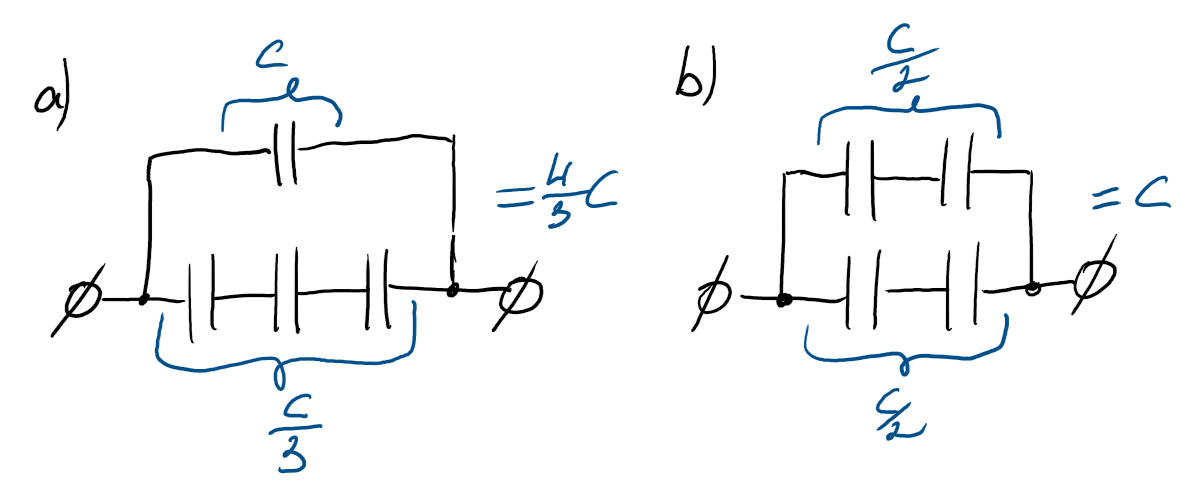
\includegraphics[width=0.9\textwidth]{physics1/images/physics1_homework_8_1}
\end{center}

Обозначим $C$ емкостью конденсатора, тогда в схеме a) нижние конденсаторы 
соединены последовательно и образуют емкость $\frac{1}{\frac{1}{C} + \frac{1}{C} + \frac{1}{C}} = \frac{C}{3}$ - 
эта группа соединена параллельна с верхним конденсатором, тогда емкость батареи - $C + \frac{C}{3} = \frac{4}{3}C$

Аналогично в схеме b) емкость батареи будет $2\left(\frac{1}{\frac{1}{C} + \frac{1}{C}}\right) = C$

Очевидно, что в схеме a) емкость больше, чем в схеме b)

\mediumvspace

Выясним, при каком соотношении емкость батареи в двух конфигурациях будет равна:

$\frac{1}{\frac{1}{C_1} + \frac{1}{C_2} + \frac{1}{C_3}} + C_4 = \frac{1}{\frac{1}{C_1} + \frac{1}{C_2}} + \frac{1}{\frac{1}{C_3} + \frac{1}{C_4}}$

$\frac{C_1 C_2 C_3}{C_2 C_3 + C_1 C_3 + C_1 C_2} + C_4 = \frac{C_1 C_2}{C_1 + C_2} + \frac{C_3 C_4}{C_3 + C_4}$

$C_1 C_2 \frac{C_3 C_1 + C_3 C_2 - C_2 C_3 - C_1 C_3 - C_1 C_2}{C_2 C_3 + C_1 C_3 + C_1 C_2} = -\frac{C^2_4}{C_3 + C_4}$

$\frac{C^2_1 C^2_2}{C_2 C_3 + C_1 C_3 + C_1 C_2} = \frac{C^2_4}{C_3 + C_4}$


\bigvspace

\underline{Ответ}: $\frac{C^2_1 C^2_2}{C_2 C_3 + C_1 C_3 + C_1 C_2} = \frac{C^2_4}{C_3 + C_4}$

\begin{tcolorbox}
    \textbf{Задача 13.9.} Четыре одинаковых конденсатора 
    соединены и присоединены к батарее с ЭДС $\varepsilon$.
    Ключ $K_2$ сначала разомкнут, а ключ $K_1$ замкнут. 
    Затем размыкают ключ $K_1$ и замыкают
    ключ $K_2$. Какова будет разность потенциалов
    на каждом конденсаторе, если ЭДС батареи
    $\varepsilon = 9$ В?
\end{tcolorbox}

\begin{minipage}{\textwidth}
    \begin{wrapfigure}{r}{0pt}
        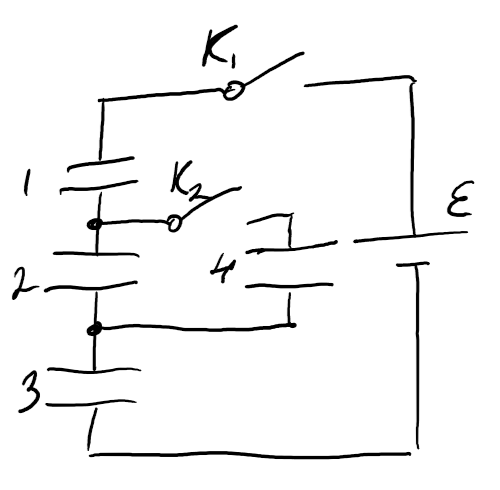
\includegraphics[width=0.4\textwidth]{physics1/images/physics1_homework_8_2}
    \end{wrapfigure}

    Ключ $K_1$ замкнут, значит через конденсаторы 1, 2 и 3 идет ток. Через конденсатор 4 ток не идет, так как ключ $K_2$ разомкнут.
    Всего емкость трех конденсаторов равна $C_{123} = \frac{C}{3}$, где $C$ - емкость одного конденсатора. Разность потенциала между ними $\varphi =$ 9 вольт,
    так как конденсаторы соединены последовательно, заряд на всех конденсаторах будет $q_1 = q_2 = q_3 = C_{123} \varphi = 3C$,
    а напряжение $U_1 = \frac{q_1}{C} = 3$ В
    
    Будем считать четвертый конденсатор незаряженным; при размыкании ключа $K_1$ ничего не происходит, при замыкании ключа $K_2$ ток пойдет
    от второго конденсатора к четвертому, причем $U_{2\text{после}} = U_{4} = \frac{U_{2\text{до}}}{2} = 1.5$ В

    Первый и третий конденсаторы не подключены в цепь, напряжение на них не изменится
\end{minipage}

\bigvspace

\underline{Ответ}: 3 В, 1.5 В, 3 В, 1.5 В

\begin{tcolorbox}
    \textbf{Задача 9.3.4.} Пространство между
    обкладками плоского конденсатора заполнено двумя
    слоями диэлектриков. Толщина слоя первого диэлектрика с
    проницаемостью $\varepsilon_1$ равна $h_1$, толщина
    слоя второго диэлектрика с проницаемостью $\varepsilon_2$ равна $h_2$. 
    Площадь каждой обкладки равна S. Найти емкость $C$ конденсатора.
\end{tcolorbox}

\begin{minipage}{\textwidth}
    \begin{wrapfigure}{r}{0pt}
        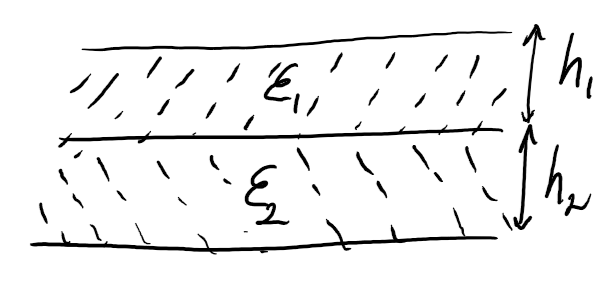
\includegraphics[width=0.4\textwidth]{physics1/images/physics1_homework_8_3}
    \end{wrapfigure}

    Считаем конденсаторы соединенными последовательно, тогда 

    $C = \frac{1}{\frac{1}{C_1} + \frac{1}{C_2}} = \frac{1}{\frac{h_1}{\varepsilon \varepsilon_1 S} + \frac{h_2}{\varepsilon \varepsilon_2 S}} = 
    \frac{1}{\frac{h_1 \varepsilon_2 + h_2 \varepsilon_1}{\varepsilon \varepsilon_1 \varepsilon_2 S}} = \frac{\varepsilon \varepsilon_1 \varepsilon_2 S}{h_1 \varepsilon_2 + h_2 \varepsilon_1}$
\end{minipage}

\bigvspace

\underline{Ответ}: $\frac{\varepsilon \varepsilon_1 \varepsilon_2 S}{h_1 \varepsilon_2 + h_2 \varepsilon_1}$

\begin{tcolorbox}
    \textbf{Задача 11.3.9.} Плоский воздушный конденсатор с пластинами
    площадью $S$ и расстоянием между ними $d$ заряжен до разности потенциалов $U$ и отключен от батареи. Какую минимальную работу
    надо совершить, чтобы увеличить расстояние между его пластинами на $\Delta x$?
\end{tcolorbox}


\begin{minipage}{\textwidth}
    \begin{wrapfigure}{r}{0pt}
        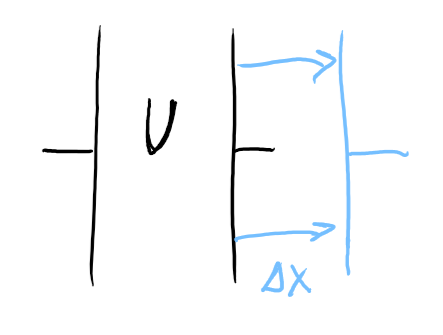
\includegraphics[width=5cm]{physics1/images/physics1_homework_8_4}
    \end{wrapfigure}

    В ходе перемещения обкладки заряд на конденсаторе не изменяется, поэтому $q = \mathrm{const} = CU = \frac{\varepsilon \varepsilon_0 S}{d} U$

    Тогда $\frac{\varepsilon \varepsilon_0 S}{d} U = \frac{\varepsilon \varepsilon_0 S}{d + \Delta x} U^{\prime}$

    Из этого $U^\prime = \frac{d + \Delta x}{d} U$

    Получаем разность напряжений $\Delta U = U^\prime - U = U\left(\frac{d + \Delta x}{d} - 1\right) = U \frac{\Delta x}{d}$

    Получаем работу $A = q \Delta U = q U \frac{\Delta x}{d} = \frac{\varepsilon \varepsilon_0 S \Delta x}{d^2} U^2$

\end{minipage}

\bigvspace

\underline{Ответ}: $\frac{\varepsilon \varepsilon_0 S \Delta x}{d^2} U^2$ Дж

\begin{tcolorbox}
    \textbf{Задача 11.3.13.} Конденсатор емкости $C_1 = 1$ мкФ ($10^{-6}$ Ф), предварительно 
    заряженный до напряжения $U = 300$ В и отсоединенный от
    источника ЭДС, подключили параллельно к незаряженному конденсатору емкости $C_2 = 2$ мкФ. 
    Найти изменение энергии этой системы к моменту установления равновесия.
\end{tcolorbox}

\begin{minipage}{\textwidth}
    \begin{wrapfigure}{r}{0pt}
        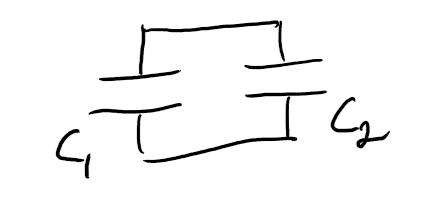
\includegraphics[width=5cm]{physics1/images/physics1_homework_8_5}
    \end{wrapfigure}

    Конденсаторы соединены параллельно, значит $U_1 = U_2$

    На первом конденсаторе до подключения ко второму сосредоточился заряд $Q = C_1 \cdot U$

    По закону сохранения заряда $q_2 + q_1 = Q \Longrightarrow C_1 U_1 + C_2 U_2 = C_1 \cdot U$

    $U_1 = U_2 = \frac{C_1}{C_1 + C_2} U$

    Энергия первого конденсатора до подключения ко второму равна $W_1 = \frac{C_1 U^2}{2} = \frac{10^{-6} \cdot 90000}{2} = 0.045$ Дж; 
    после подключения $W_2 = \frac{C_1 U_1^2 + C_2 U_2^2}{2} = \frac{C_1 + C_2}{2} \frac{C^2_1}{(C_1 + C_2)^2} U^2 = 
    \frac{C^2_1}{2(C_1 + C_2)} U^2 = \frac{10^{-12}}{2 (10^{-6} + 2 \cdot 10^{-6})} \cdot 90000 = \frac{10^{-6}}{6} \cdot 90000 = 0.015$ Дж

    $\Delta W = -0.03$ Дж

\end{minipage}

\bigvspace

\underline{Ответ}: -0.03 Дж


% end physics1_homework_8.tex

% begin physics1_homework_9.tex





\begin{tcolorbox}
    \textbf{Задача 2.3.5} Сила тока $I(t)$ в проводнике меняется со временем $t$ по
    уравнению $I(t) = 4 + 2t$, где $I$ выражено в амперах и $t$
    в секундах.

    \begin{enumerate}
        \item Какое количество электричества проходит через поперечное сечение
        проводника за время от $t_1 = 2$ с до $t_2 = 6$ с? 
        \item При какой силе постоянного тока через поперечное сечение 
        проводника за это же время проходит
        такое же количество электричества?
    \end{enumerate}

    \begin{UpsideDown}
        \footnotesize
        \underline{Ответ}: 48 Кл, 12 А.
    \end{UpsideDown}
\end{tcolorbox}

Количество заряда за промежуток времени $dt$ определяется как $dq = I dt$, тогда $q = \int_2^6 Idt = 4t + t^2 \Big|_2^6 = 48$

При $I = \mathrm{const}$ получаем, что $I = \frac{q}{t} = \frac{48}{4} = 12$

\bigvspace

\underline{Ответ}: 48 Кл, 12 А.

\begin{tcolorbox}
    \textbf{Задача 2.3.15} Из кусочка алюминия массой $m = 21.2$ г изготавливают
    цилиндрический провод длиной $l = 10$ м. Найти его сопротивление. Каков диаметр провода? 
    Плотность алюминия $\rho_m = 2.70 \cdot 10^3$ кг/мз.

    \begin{UpsideDown}
        \footnotesize
        \underline{Ответ}: 0.32 Ом, 1 мм.
    \end{UpsideDown}
\end{tcolorbox}

Удельное сопротивление алюминия $\rho_R = 0.028 \frac{\text{Ом} \cdot \text{мм}^2}{\text{м}} = 2.8 \cdot 10^{-8} \text{Ом} \cdot \text{м}$

Сопротивление проводника вычисляется по формуле $R = \frac{\rho_R l}{S} = \frac{\rho_R l}{\frac{V}{l}} = \frac{\rho_R l^2 \rho}{m} = 
\frac{2.8 \cdot 10^{-8} \cdot 10^2 \cdot 2.7 \cdot 10^3}{0.0212} = 0.356$ Ом

Диаметр проводника $d = 2r = 2\sqrt{\frac{S}{\pi}} = 2\sqrt{\frac{m}{\pi \rho l}} = 1 \cdot 10^{-3} \ \text{м} = 1 \ \text{мм}$

\bigvspace

\underline{Ответ}: 0.356 Ом, 1 мм.

\begin{tcolorbox}
    \textbf{Задача 2.3.26} Две батареи с ЭДС $\varepsilon_1 = 20$ В, $\varepsilon_2 = 30$ В и внутренним
    сопротивлением $r_1 = 4$ Ом, $r_2 = 6$ Ом соединены параллельно. Каковы
    ЭДС и внутреннее сопротивление источника тока, которым можно заменить 
    эти батареи без изменения тока в нагрузке?

    \begin{UpsideDown}
        \footnotesize
        \underline{Ответ}: 24 В, 2.4 Ом.
    \end{UpsideDown}
\end{tcolorbox}

Источники тока соединены параллельно, тогда их общее внутреннее сопротивление $r = \frac{r_1 r_2}{r_1 + r_2} = \frac{4 \cdot 6}{10}= 2.4$ Ом

Общая сила тока источников равна $I = I_1 + I_2 = \frac{\varepsilon_1}{r_1} + \frac{\varepsilon_2}{r_2} = 10$ А

Тогда у заменяющей батареи должна быть ЭДС $\varepsilon = Ir = 24$ В

\bigvspace

\underline{Ответ}: $24$ В, $2.4$ Ом.


\begin{tcolorbox}
    \textbf{Задача 2.3.56} Аккумулятор замыкается один раз на сопротивление $R_1 = 20$ Ом, 
    другой раз - на сопротивление $R_2 = 5$ Ом. При этом количество
    тепла, выделяющееся во внешней цепи в единицу времени, одинаково.
    Найти внутреннее сопротивление аккумулятора.
    
    \begin{UpsideDown}
        \footnotesize
        \underline{Ответ}: 10 Ом.
    \end{UpsideDown}
\end{tcolorbox}

По закону Джоуля-Ленца $Q = I_1^2 R_1 \Delta t = I_2^2 R_2 \Delta t$, где $I_1 = \frac{\varepsilon}{R_1 + r}$, $I_2 = \frac{\varepsilon}{R_2 + r}$

Получаем $\fraC{\varepsilon^2 R_1}{(R_1 + r)^2} = \frac{\varepsilon^2 R_2}{(R_2 + r)^2}$

$(R_2 + r)^2 \cdot R_1 = (R_1 + r)^2 \cdot R_2 \Longrightarrow 100 + 40r + 4r^2 = 400 + 40r + r^2 \Longrightarrow r = 10$

\bigvspace

\underline{Ответ}: 10 Ом.

% end physics1_homework_9.tex



\end{document}

